%% One source, two builds (see Makefile):
%%   anonymous ECIR 2027 submission  -> default
%%   de-anonymised arXiv preprint    -> \def\arxiv{} before %% One source, two builds (see Makefile):
%%   anonymous ECIR 2027 submission  -> default
%%   de-anonymised arXiv preprint    -> \def\arxiv{} before %% One source, two builds (see Makefile):
%%   anonymous ECIR 2027 submission  -> default
%%   de-anonymised arXiv preprint    -> \def\arxiv{} before %% One source, two builds (see Makefile):
%%   anonymous ECIR 2027 submission  -> default
%%   de-anonymised arXiv preprint    -> \def\arxiv{} before \input{main}
\documentclass[runningheads]{llncs}

\usepackage[T1]{fontenc}
\usepackage{lmodern}
\usepackage{booktabs}
\usepackage{amsmath}
\usepackage{amssymb}
\usepackage{graphicx}
\usepackage{xcolor}
\usepackage{tikz}
\usetikzlibrary{positioning, arrows.meta, shapes.geometric,
                fit, backgrounds, calc}
\usepackage{cite}
\usepackage{microtype}
\usepackage[hidelinks]{hyperref}

\newif\ifanonymous
\ifdefined\arxiv \anonymousfalse \else \anonymoustrue \fi

%% acmart's accessibility description; LNCS has no equivalent.
\newcommand{\Description}[1]{}

\begin{document}

\title{A Multi-Axis Robustness Analysis of Retrieval-Augmented Generation
  for Multi-Hop Requirements Traceability}
\titlerunning{Multi-Axis Robustness of RAG for Requirements Traceability}

\ifanonymous
\author{Anonymous Author(s)}
\authorrunning{Anonymous}
\institute{Anonymous Institution}
\else
\author{Meftun Akarsu\inst{1} \and
  Burak \"Ozdemir\inst{1} \and
  Do\u{g}ancan B\"uy\"uk\c{c}olak\inst{1} \and
  Recep Kaan Karaman\inst{2}}
\authorrunning{M. Akarsu et al.}
\institute{Turkish Aerospace Industries, Ankara, T\"urkiye \and
  Technical University of Munich, Munich, Germany\\
  \email{kaan.karaman@tum.de}}
\fi

\maketitle

\input{sections/01-abstract}
\input{sections/02-introduction}
\input{sections/03-related-work}
\input{sections/04-method}
\input{sections/05-experiments}
\input{sections/06-results}
\input{sections/07-discussion}
\input{sections/08-conclusion}

\bibliographystyle{splncs04}
\bibliography{refs}

\end{document}

\documentclass[runningheads]{llncs}

\usepackage[T1]{fontenc}
\usepackage{lmodern}
\usepackage{booktabs}
\usepackage{amsmath}
\usepackage{amssymb}
\usepackage{graphicx}
\usepackage{xcolor}
\usepackage{tikz}
\usetikzlibrary{positioning, arrows.meta, shapes.geometric,
                fit, backgrounds, calc}
\usepackage{cite}
\usepackage{microtype}
\usepackage[hidelinks]{hyperref}

\newif\ifanonymous
\ifdefined\arxiv \anonymousfalse \else \anonymoustrue \fi

%% acmart's accessibility description; LNCS has no equivalent.
\newcommand{\Description}[1]{}

\begin{document}

\title{A Multi-Axis Robustness Analysis of Retrieval-Augmented Generation
  for Multi-Hop Requirements Traceability}
\titlerunning{Multi-Axis Robustness of RAG for Requirements Traceability}

\ifanonymous
\author{Anonymous Author(s)}
\authorrunning{Anonymous}
\institute{Anonymous Institution}
\else
\author{Meftun Akarsu\inst{1} \and
  Burak \"Ozdemir\inst{1} \and
  Do\u{g}ancan B\"uy\"uk\c{c}olak\inst{1} \and
  Recep Kaan Karaman\inst{2}}
\authorrunning{M. Akarsu et al.}
\institute{Turkish Aerospace Industries, Ankara, T\"urkiye \and
  Technical University of Munich, Munich, Germany\\
  \email{kaan.karaman@tum.de}}
\fi

\maketitle

\begin{abstract}
Published comparisons of GraphRAG and vector RAG reach conflicting
verdicts, and each typically rests on a single corpus, embedder, and
judge. We hold five RAG pipelines fixed and vary the embedder, the
corpus (DO-178C requirements, MuSiQue, and 2WikiMultihopQA), the graph
traversal, and the faithfulness judge, over 13{,}456 generation runs
and more than 30{,}000 judgments. We find that the point at which
citation quality is measured decides the comparison. GraphRAG's graph
walk fills the context with mostly irrelevant chunks, at a precision of
0.12 to 0.23, while its synthesizer cites selectively. Scored on the
retrieved context, GraphRAG therefore ranks below the vanilla baseline
in all six settings we test; scored on the answer's citations, it ranks
first. The best pipeline at each hop depth is stable across embedders
and seeds. Faithfulness declines with hop depth on all three corpora
once the comparison is adequately powered, and the decline follows
context expansion: the one pipeline that does not expand its context
does not decline. LLM judges, in contrast, are unstable. On identical
inputs re-judged eleven weeks later, self-agreement falls to
$\kappa \le 0.14$, and two vendors reverse which of them is stricter
between corpora. We recommend that RAG architecture comparisons report
the citation measurement point and be repeated across these factors.

\keywords{Retrieval-augmented generation \and GraphRAG \and Requirements traceability \and Multi-hop QA \and LLM-as-judge \and Evaluation methodology}
\end{abstract}

\section{Introduction}
\label{sec:intro}

Software traceability is the ability to relate each requirement to the
artifacts it derives from, satisfies, and is verified by. For airborne
software, DO-178C makes this relation a certification objective, and
certification authorities increasingly expect trace chains to be
auditable across two or more hops~\cite{do178c,arp4754a,easa2025npa,faa2024airoadmap}.
Because requirements management tools record these links explicitly, a
requirements corpus is also a typed link graph, and answering a
traceability question over it is a retrieval problem over both text and
graph.

Retrieval-augmented generation (RAG) is a natural fit for this task,
but published comparisons of RAG architectures disagree. Microsoft
GraphRAG~\cite{graphrag2024} exploits graph structure, yet loses to
vector RAG on detailed queries in recent
benchmarks~\cite{ragvsgraphrag2025,graphragbench2026}.
Adaptive-RAG~\cite{adaptiverag2024} routes queries by predicted
complexity but does not consider hop distance, and traceability systems
such as LiSSA~\cite{lissa2025} and TVR~\cite{niu_tvr2025} do not reason
over typed graphs. Each of these evaluations reports which architecture
wins in one setting, usually with one corpus, one embedder, and one
judge. They do not explain why the verdict changes when the setting
changes.

In this paper, we hold a matrix of five pipelines fixed (vanilla,
agentic, agentic with a graph tool, GraphRAG, and a learned adaptive
router) and vary four factors around it. These are the retrieval
embedder (e5-small, OpenAI text-embedding-3-small, and bge-m3, from
three vendors and at three dimensionalities), the corpus (DO-178C
requirements with typed edges, and Wikipedia paragraph chains from
MuSiQue and 2WikiMultihopQA), the graph traversal (a bounded two-hop
walk and personalized PageRank), and the faithfulness judge (GPT-5.4,
GPT-4.1, and Gemini 3.7-flash). The design comprises 13{,}456 generation
runs and more than 30{,}000 faithfulness judgments. We ask four research questions. \textbf{RQ1}: Which
pipeline produces the best answer-level citations at each hop depth,
and is that ordering stable across embedders, corpora, and seeds?
\textbf{RQ2}: Does the GraphRAG versus vector RAG comparison depend on
whether citation quality is measured on the retrieved context or on the
answer? \textbf{RQ3}: Does faithfulness decline with hop depth on every
corpus, and which property of a pipeline determines the decline?
\textbf{RQ4}: How stable are LLM faithfulness judges across time,
retrieval states, and vendors?

We find that the best pipeline depends on hop depth but not on the
embedder or the seed (RQ1); that GraphRAG ranks below the vanilla
baseline when citations are scored on the retrieved context and first
when they are scored on the answer, in all six settings we test (RQ2);
that faithfulness declines with hop depth on all three corpora once
adequately powered, and only for pipelines that expand their context
(RQ3); and that judges drift on identical inputs and reverse which of
them is stricter between corpora, while reproducing the same hop-wise
ordering (RQ4).

\section{Related Work}
\label{sec:related}

\paragraph{Agentic and adaptive RAG.}
Self-RAG~\cite{selfrag2024} and CRAG~\cite{crag2024} introduced
reflective and corrective retrieval. Adaptive-RAG~\cite{adaptiverag2024}
routes queries by predicted complexity, and
Probing-RAG~\cite{probingrag2025} extends this idea with probes on the
model's internal states. Search-R1~\cite{searchr1_2025} trains agentic
retrieval with reinforcement learning, and RAG-Critic~\cite{ragcritic2025}
adds an iterative critic. None of these methods conditions routing on
hop distance in a typed graph or exposes a typed graph-lookup tool.

\paragraph{GraphRAG and multi-hop QA.}
Microsoft GraphRAG~\cite{graphrag2024} and its
successors~\cite{lightrag2024,hipporag2_2025,graphr1_2025} build
entity--relation graphs at indexing time. Han et al.~\cite{ragvsgraphrag2025}
and GraphRAG-Bench~\cite{graphragbench2026} report that GraphRAG does
not outperform vector RAG on every query type. Our RQ2 results suggest one reason such verdicts differ: whether
citations are scored on the retrieved set or on the answer. Of the multi-hop benchmarks MuSiQue~\cite{musique2022},
MultiHop-RAG~\cite{multihoprag2024}, and
2WikiMultihopQA~\cite{twowiki2020}, we use the first and last to test
RQ1 to RQ3 outside the requirements domain.

\paragraph{RAG for requirements traceability.}
LiSSA~\cite{lissa2025}, TVR~\cite{niu_tvr2025}, and Graph-RAG for
compliance checking~\cite{graphragcompliance2024} each evaluate a single
regulated domain, without stratifying queries by hop depth and with a
single judge.

\paragraph{Citation evaluation and judge reliability.}
ALCE~\cite{alce2023} defined citation precision, recall, and $F_1$ for
generated answers. Wallat et al.~\cite{wallat2024} show that ALCE-style
correctness does not imply faithfulness, which motivates the use of LLM
judges. RAGChecker~\cite{ragchecker2024} provides a single-judge
framework, and self-preference bias~\cite{selfpref_bias2024} motivates
judge ensembles. Feinstein and Cicchetti~\cite{feinstein1990} describe
the prevalence paradox of Cohen's $\kappa$, and Gwet's
AC1~\cite{gwet2008} is the correction we report alongside it. Our
analysis for RQ4 adds a quantity this literature does not track, the
agreement of a judge with its own earlier verdicts after the retrieval
state or the date changes.

\section{Method}
\label{sec:method}

\begin{figure}[t!]
  \centering
  \resizebox{0.36\textwidth}{!}{\input{figures/architecture-tikz}}%
  \caption{The five pipelines and their shared components. Vanilla and
    GraphRAG make a single synthesis call. Agentic and Agentic+Graph run
    a router, retriever, tool, and critic loop for at most three
    iterations before synthesis. The adaptive pipeline (rule-based V1 or
    learned V2) selects one of the four base pipelines per query.}
  \label{fig:architecture}
\end{figure}

\subsection{Pipelines}
\label{sec:pipelines}
All pipelines share the embedder, a ChromaDB vector store, a file-backed
typed-edge graph, the GPT-5.4 generator, and a grounded synthesis
prompt, so they differ only in how they retrieve
(Fig.~\ref{fig:architecture}).
\textbf{(i)~Vanilla} retrieves the top 10 chunks by dense similarity,
passes the top 5 to the synthesizer, and makes one synthesis call.
\textbf{(ii)~Agentic} is a LangGraph~\cite{langgraph_software} loop of
router, retriever, and critic with a single \texttt{search\_documents}
tool and at most three iterations.
\textbf{(iii)~GraphRAG} takes 8 vector seeds, walks up to two hops in
the typed graph (at most 30 nodes), and passes at most 15 chunks to one
synthesis call. It is a local-walk retriever in the GraphRAG family
rather than the community-summarisation system of Edge
et al.~\cite{graphrag2024}; we use ``GraphRAG'' as the family name.
\textbf{(iv)~Agentic+Graph} adds a typed \texttt{graph\_lookup} tool to
(ii). \textbf{(v)~Adaptive} chooses among (i) to (iv) for each query. We
evaluate a rule-based router (V1) and a learned router (V2), an
out-of-fold logistic regression over 11 text features and 3
principal components of the query embedding that sends each predicted
hop class to its empirically best pipeline.

\subsection{Experimental Factors}
\label{sec:axes}
\textbf{Embedder.} We use three models from three vendors at three
dimensionalities: e5-small (384 dimensions), OpenAI
text-embedding-3-small (1536), and BAAI bge-m3 (1024). The vector index is rebuilt per embedder; the graph is shared.
\textbf{Traversal.} Besides the bounded undirected walk (at most two
hops, at most 30 nodes), we run personalized PageRank from the same
vector seeds. It is unbounded in radius and ranks nodes by random-walk
mass, and all other settings are held fixed.
\textbf{Corpus.} The main corpus is a synthetic DO-178C-style
collection of 1{,}132 aerospace requirements in 30 modules (17 to 76
requirements per module; median length 59 tokens, 90th percentile 103).
GPT-5.4 generated it from a hand-authored module taxonomy, and we
release it with its link annotations. Retrieval traverses five
traceability edge types (\textit{derives\_from}, \textit{satisfies},
\textit{references}, \textit{verifies}, and \textit{refines}); we exclude
system-engineering edges such as allocation, which do not help
retrieval. Two Wikipedia corpora test transfer: 200 MuSiQue~\cite{musique2022}
questions (67, 67, and 66 of two, three, and four hops, mapped to our
three strata, with \textit{REFERENCES} edges between consecutive
supporting paragraphs) and 200 2WikiMultihopQA~\cite{twowiki2020}
questions, stratified by reasoning type: \textit{comparison} questions are one-hop,
\textit{compositional} and \textit{inference} questions are two-hop, and
\textit{bridge\_comparison} questions are three-or-more-hop.
\textbf{Judge.} Faithfulness is judged by GPT-5.4, GPT-4.1, and
Gemini 3.7-flash (Section~\ref{sec:experiments}).

\subsection{Queries and Gold Evidence}
\label{sec:queries}
We build the DO-178C queries from the graph rather than by free-form
prompting. We sample directed chains of one, two, and three to four
requirement links over the five edge types and prompt GPT-5.4 to phrase
one natural-language question that the chain answers. The nodes of the
chain form the gold evidence, so the gold set grows with the stratum
(on average 2.00, 3.00, and 4.68 IDs). This yields 296 queries (100,
99, and 97 per stratum), of which 85\% cross module boundaries; 497 of
the 655 chain edges are \textit{references} links. The gold sets are structural rather than human-annotated: a sampled
chain is a supporting path by construction, but we do not verify that
no other path answers the question. Citation recall is therefore exact
and precision conservative, equally for all pipelines.

\subsection{Metrics}
\label{sec:metrics}
We report citation precision, recall, and $F_1$ against the gold ID
sets, following ALCE~\cite{alce2023}. Cited IDs are parsed from the
answer text with a parser anchored to the corpus vocabulary, which
matches exact IDs and prefers the longest match. Hallucinated IDs that
reuse a real module prefix count against precision, and incidental
tokens such as SHA-256 or DO-254 are ignored. We report separately the context precision (the gold fraction of the
chunks handed to the synthesizer) and the retrieval recall, since
conflating context and citations changes which architecture appears to
win (Section~\ref{sec:c2}).

Each faithfulness judgment is a binary verdict, returned as strict JSON,
on whether the answer is supported by the retrieved context. For
agreement we report Cohen's $\kappa$, Gwet's
AC1~\cite{gwet2008,feinstein1990}, raw agreement, and an exact McNemar
test. For each faithfulness cell we report a Wilson 95\% confidence
interval and a Cochran--Armitage test for trend over hop depth. Three
same-judge controls (test--retest, embedder swap, and re-judging after
eleven weeks) use a paired subset of 300 tuples
(Section~\ref{sec:c4}).

\section{Experimental Setup}
\label{sec:experiments}

\noindent\textbf{Runs.} On DO-178C, we run 5 pipelines $\times$ 296 queries
$\times$ 3 seeds, giving 4{,}440 runs under each of two embedders
(e5-small, which we call \emph{v2}, and text-embedding-3-small,
\emph{v3}). We add 1{,}480 runs at one seed under bge-m3 (\emph{v4})
and a 296-run personalized PageRank arm under the v3 embedder. On
MuSiQue, we run vanilla, GraphRAG, and agentic+graph on 200 queries at
one seed (600 runs, v3 embedder), since RQ2 needs only these three, and
extend the GraphRAG arm to three seeds to match DO-178C's per-stratum
sample. On the same queries we add 400 runs for two mitigations and a
200-run GraphRAG control with distractor edges (Section~\ref{sec:c1}).
On 2WikiMultihopQA, we run vanilla and GraphRAG on 200 queries at three
seeds (1{,}200 runs, v3 embedder).

\noindent\textbf{Faithfulness judging.} On DO-178C, GPT-5.4 and GPT-4.1 judge
two disjoint stratified batches of 300 rows each (60 per pipeline;
seeds 42 and 43), the second eleven weeks after the first. Each batch is
fixed to the same 300 (query, pipeline, repeat) tuples across
embedders, so embedder differences are computed on identical items, and
batches judged on different dates are never pooled. In a later pass, GPT-4.1
and Gemini 3.7-flash judge every row of the DO-178C matrices and of the
Wikipedia corpora. Gemini judged four days after GPT-4.1 on DO-178C and
one day after it on the Wikipedia corpora, in both cases on the same
stored answer and context strings, so the pairing is exact at the row
level. Two same-input
controls re-judge 300 v2 tuples with GPT-5.4, once on the same day
(test--retest) and once eleven weeks later. A generator-swap control
re-synthesizes 332 v3 rows with GPT-4.1 on frozen retrievals and judges
them with both judges.

\noindent\textbf{Statistical protocol.} We compute 95\% BCa bootstrap
intervals~\cite{du2025bootstrap} with 1{,}000 resamples paired at the
query level, Wilcoxon signed-rank tests with Holm correction over the
30 contrasts of pipeline pair and stratum~\cite{bergkirkpatrick2012,koehn2004},
and Cliff's $\delta$, which we treat as negligible below 0.147. We call
two pipelines significantly different only when the BCa interval
excludes zero, the Holm-adjusted $p$ is below 0.05, and
$|\delta| \ge 0.147$. Tests pool the three seeds; we report the spread across seeds
separately (Section~\ref{sec:c1}).

\noindent\textbf{Reproducibility.} The original graph store was populated
before this study and contains edges beyond those annotated in the
released corpus. Loading the release with our ETL recovers 91.0\% of
the edges and 82.8\% of the chains behind our queries. Every gold set is
nevertheless exact, since the query manifest is released with its full
chains. The v2 and v3 graph arms walked the original store, while
the bge-m3 matrix and the PageRank arm walked a file-backed store built
from the released annotations, which is also what a reproduction uses.
To check that the change of graph does not drive our comparisons, we
rebuilt every v3 GraphRAG context on the file-backed store without
generation. The vector seeds are identical for 295 of the 296 queries,
the two contexts have a Jaccard overlap of 0.89, and context precision
(0.131 against 0.129) and retrieval recall (0.720 against 0.724) differ
by at most 0.01 in every stratum. We did not regenerate answers on the
new store, so the citation side of this check is untested.
We use the Azure snapshots \texttt{gpt-5.4-}\allowbreak\texttt{2026-03-05}
(generator and judge) and \texttt{gpt-4.1-2025-04-14} (judge) in
reasoning mode, with a completion cap of 8{,}192 tokens. The MuSiQue
subgraph (3{,}996 paragraph chunks and 399 \textit{REFERENCES} edges) is
built deterministically from the \texttt{dgslibisey} mirror (validation
split, seed 20260511), and the 2WikiMultihopQA subgraph (2{,}000 chunks
and 332 edges) from the \texttt{voidful} mirror (seed 20260816) by the
same procedure.

\section{Results}
\label{sec:results}

\input{tables/tab_dominance}

\begin{figure}[t!]
  \centering
  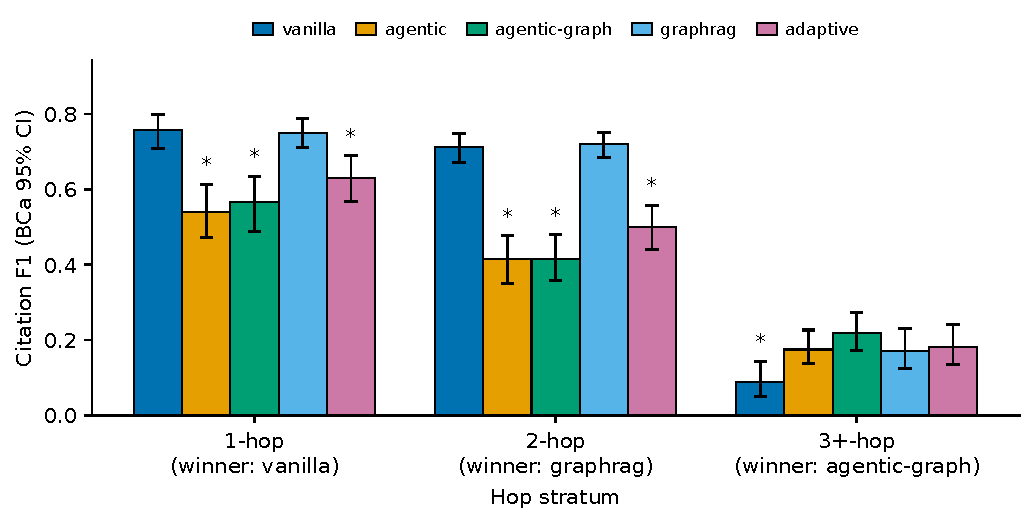
\includegraphics[width=0.55\textwidth]{figures/fig1_per_stratum_f1.pdf}
  \caption{Citation $F_1$ by hop stratum on the v2 matrix (DO-178C,
    e5-small), with 95\% BCa intervals. An asterisk marks a pipeline that
    differs significantly from the best pipeline in its stratum (Holm-adjusted
    Wilcoxon $p < 0.05$ and $|\delta| \ge 0.147$).}
  \label{fig:perstratum}
\end{figure}

\subsection{Citation Quality by Hop Depth (RQ1)}
\label{sec:c1}
Table~\ref{tab:dominance} reports citation $F_1$ by stratum in four
settings. On DO-178C, vanilla and GraphRAG are statistically tied on
one- and two-hop queries (Wilcoxon $p = 0.12$ and $0.65$ under the v2
embedder, with negligible $\delta$), and the agentic loop costs 0.19 to
0.30 $F_1$ on these strata. On queries of three or more hops the
ordering reverses. Vanilla falls to last place, and the pipelines that
use the graph lead; under the v2 embedder agentic+graph reaches 0.219
against 0.089 for vanilla (Holm $p < 10^{-6}$). Under the v3 embedder the ordering is the same, but no pair at this depth passes the joint criterion. Under bge-m3 the pattern recurs (Table~\ref{tab:embedders}):
vanilla is last at three or more
hops under all three embedders, and under bge-m3 both graph pipelines
outperform it by 0.100 and 0.091 (Holm $p = 2.1 \times 10^{-4}$ and
$1.4 \times 10^{-3}$), while the one- and two-hop contrasts remain
negligible.

On MuSiQue, GraphRAG is best in every stratum ($F_1$ of 0.841, 0.632,
and 0.463), with $p \le 5.1 \times 10^{-4}$ and $\delta$ between 0.27
and 0.43 against vanilla. Because the MuSiQue \textit{REFERENCES} edges
connect only gold paragraphs, we also ran GraphRAG on a graph with
additional edges between consecutive distractor paragraphs. GraphRAG
then loses 0.02, 0.05, and 0.09 $F_1$ per stratum and still outperforms
vanilla in every stratum ($p \le 0.014$), so its advantage on MuSiQue
does not depend on gold-only edges. On 2WikiMultihopQA, the two
pipelines are tied on one-hop queries ($p = 0.15$), and GraphRAG leads
on two-hop and deeper queries by 0.168 and 0.260 ($\delta = 0.48$ and
0.87). This is the DO-178C crossover again, on a graph we did not build.

Seed variation is small by comparison. The mean $F_1$ of each pipeline
changes by at most 0.031 between seeds,
every significant ordering holds in each seed separately, and the only
changes in rank occur between vanilla and GraphRAG on one- and two-hop
queries, which we already report as ties. Regarding RQ1, the best
pipeline depends on hop depth and on the corpus, but not on the embedder
or the seed.

\input{tables/tab_embedders}

\input{tables/tab_pathology}

\begin{figure}[t!]
  \centering
  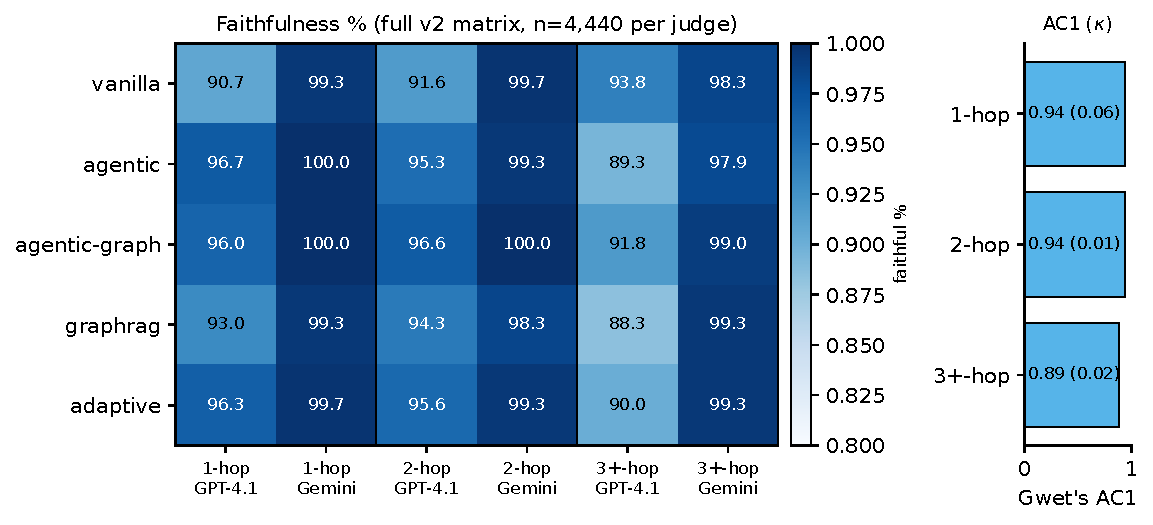
\includegraphics[width=0.8\textwidth]{figures/fig2_faithfulness_heatmap.pdf}
  \caption{Faithfulness on the full v2 matrix (DO-178C, e5-small; 4{,}440
    rows, about 300 per cell), judged by GPT-4.1 and Gemini 3.7-flash on
    the same rows. Left: percentage of answers judged faithful. Right:
    Gwet's AC1 between the two judges per stratum, with Cohen's $\kappa$
    in parentheses. The colour scale starts at 80\%.}
  \label{fig:faithheatmap}
\end{figure}

\subsection{Context Versus Answer Citations (RQ2)}
\label{sec:c2}
Table~\ref{tab:pathology} reports the same measurement in six settings,
covering three embedders, three corpora, and two traversals. GraphRAG's
walk fills 11 to 15 context slots at a context precision of 0.12 to
0.23, so four or five of every six chunks it retrieves are not gold. The
synthesizer then cites only 2.5 to 5.0 IDs per answer, at a citation
precision of 0.48 to 0.98. In every setting, the precision of the
citations is 2.9 to 4.2 times that of the context. The $F_1$ advantage
of GraphRAG is therefore a recall effect: the walk retrieves gold chunks
that dense retrieval misses, and the synthesizer does not cite most of
the irrelevant chunks that come with them.

An evaluation that scores the retrieved set as the attribution set, as
some GraphRAG comparisons do, sees only the first step and reaches the
opposite ranking. By context precision, GraphRAG
is below the vanilla baseline in every setting (0.12 to 0.23, against
0.27 to 0.37 for vanilla). By citation $F_1$, it is the best pipeline in
every setting, with scores of 0.551, 0.571, 0.565, 0.585, 0.646, and
0.951 in the row order of Table~\ref{tab:pathology}. 

Two controls test whether this depends on our design. The first
replaces the two-hop walk with personalized PageRank over the same
graph. Context
precision is 0.131 with PageRank and 0.129 with the original walk (0.131
for the walk rebuilt on the same file-backed graph;
Section~\ref{sec:experiments}). The precision gain from context to
citations is 3.9 and 3.8 times, and the difference in citation $F_1$ is
0.016 with $\delta = 0.036$, which our criterion treats as negligible.
The second control applies two mitigations on MuSiQue. Reranking the
walked neighbours by similarity to the query and keeping the top five
changes little (context precision from 0.227 to 0.232, citation $F_1$
$+0.010$, $p = 0.34$). Reducing the traversal budget from 30 to 10 nodes
and the context from 15 to 8 chunks lowers citation $F_1$ by 0.126
($p = 2.6 \times 10^{-11}$) and also lowers context precision, to 0.194.
Both outcomes fit a synthesizer that already filters: an upstream
filter adds little, and a smaller budget removes the recall the
advantage depends on. Regarding RQ2, the comparison
reverses with the measurement point in all six settings.

\subsection{Faithfulness and Hop Depth (RQ3)}
\label{sec:c3}
On 300-row judged subsets, faithfulness declines with hop depth on
DO-178C but not on the Wikipedia chains. This difference disappears at
adequate power. The MuSiQue arm had 67 rows per
stratum. Its drop from one-hop to three-or-more-hop queries (9.2
percentage points) was larger than the 4.7-point drop that is
significant on DO-178C, but detecting it with 80\% power requires about
210 rows per cell. With three seeds ($n = 600$), the decline is
significant under both judges, from 0.930 to 0.876 to 0.823 under GPT-4.1
($p = 1.1 \times 10^{-3}$) and from 0.955 to 0.945 to 0.869 under Gemini
($p = 1.2 \times 10^{-3}$). On 2WikiMultihopQA, judged in full
($n = 1{,}200$), faithfulness also declines ($p = 5.0 \times 10^{-2}$ and
$4.8 \times 10^{-6}$). The decline therefore replicates on all three
corpora under two vendors.

What distinguishes the pipelines is whether they expand the context.
Vanilla retrieves a fixed top five and adds nothing, and under GPT-4.1
it shows no significant drop from one-hop to three-or-more-hop queries.
Its change is $-1.5$ points on DO-178C ($n = 2{,}072$; $p = 0.16$, 0.99,
and 0.76 for the three embedders) and $+1.1$ points on 2WikiMultihopQA
($p = 0.66$). The four expanding pipelines drop by 6.3 and 6.7 points on
the same corpora (Fig.~\ref{fig:faithheatmap}). A logistic regression
of faithfulness on hop depth, an expansion indicator, and their
interaction turns this contrast into a single test. The interaction is
negative and significant on the pooled DO-178C matrix ($b = -0.599$,
$p = 1.0 \times 10^{-7}$, $n = 10{,}360$), and negative but not
significant on 2WikiMultihopQA ($b = -0.286$, $p = 0.27$), whose arm is
one twentieth the size.

Under Gemini the ordering is the same, but the test does not resolve.
Near the ceiling, vanilla itself shows a slope ($b = -0.729$,
$p = 0.012$), and the interaction cannot be separated from it
($p = 0.11$). The expanding pipelines still drop more than vanilla (2.8
against 1.5 points on DO-178C, 12.7 against 7.7 on 2WikiMultihopQA). A lenient judge preserves the ranking but not the power to test it
(Section~\ref{sec:c4}). Not every expanding pipeline declines in every cell: GraphRAG is
marginal under bge-m3 ($p = 0.065$), and the agentic pipelines decline
in four of six embedder and pipeline combinations. We have not re-run the GPT-5.4
judge at this sample size. Regarding RQ3, faithfulness declines with
hop depth on every corpus, and the decline is steeper for pipelines
that expand their context.

\input{tables/tab_judges}

\subsection{Judge Stability (RQ4)}
\label{sec:c4}
Table~\ref{tab:judges} separates instability on fixed inputs from
instability after the retrieval state changes.
\textit{Fixed inputs.} Re-judging the same 300 stored answer and
context pairs gives GPT-5.4 a self-agreement of $\kappa = 0.76$ (raw
agreement 0.88) on the same day, but only $\kappa = 0.14$ (raw agreement
0.56) eleven weeks later, with 15 points more answers judged faithful.
This rejects a stationary judge (binomial $p < 10^{-44}$). GPT-4.1 on the same tuples agrees with its own earlier
verdicts only at chance level ($\kappa = -0.05$ and $-0.00$ for v2 and
v3) and judges 41 points more answers faithful. With fixed inputs, this is drift of the judge alone.
\textit{Changed retrieval state.} After an embedder swap, which
changes the context and the answer for 94\% of the tuples, GPT-5.4
changes 41\% of its verdicts ($\kappa = 0.137$) and GPT-4.1 changes 26\%
($\kappa = 0.48$). The judge that is more stable under the embedder
swap is thus the less stable over time.
\textit{Across vendors.} On the same rows, Gemini 3.7-flash is much
more lenient than GPT-4.1 on all four DO-178C settings (0.98 to 0.99
against 0.92 to 0.95 faithful; McNemar $p < 10^{-9}$). They are indistinguishable on the budget-capped MuSiQue arm (0.875 against 0.880,
$p = 1.00$), and Gemini is stricter on 2WikiMultihopQA (0.888 against
0.914, $p = 6.2 \times 10^{-3}$). Strictness is therefore a property of
the judge and corpus together, and a calibration offset measured on one
corpus cannot be reused on another. The same eight
settings show the prevalence paradox~\cite{feinstein1990} within one
pair of judges. Raw agreement ranges only from 0.82 to 0.94, and Gwet's
AC1 follows it (0.77 to 0.94), whereas $\kappa$ ranges from 0.03 to
0.44, ordered almost exactly by the distance of faithfulness from the
ceiling. On 2WikiMultihopQA the two judges agree less often than on
DO-178C (0.899 against 0.93), yet their $\kappa$ is fifteen times
higher (0.435 against 0.029). Leniency and trend are nevertheless
separate properties. Although Gemini is near the ceiling on DO-178C, it
reproduces the decline with hop depth on both DO-178C matrices
($p = 4.3 \times 10^{-3}$ and $p < 10^{-16}$) and on both Wikipedia
corpora. The ordering a judge induces replicates across vendors, while
its strictness does not.
\textit{Between judges.} Inter-judge agreement halves under the embedder swap ($\kappa$ from
0.30 to 0.17; McNemar $p < 0.001$), and on the 300-row MuSiQue batch
GPT-5.4 and GPT-4.1 agreed only at chance (raw agreement 0.48, AC1
0.08), a real disagreement rather than a prevalence effect. We therefore
re-judged the full matrix within one judging period
(Section~\ref{sec:c3}), and no comparison we report spans judging
dates. Regarding RQ4, judges are not stable over
time, across retrieval states, or across vendors, although the hop-wise
ordering they induce is.

\section{Discussion}
\label{sec:discussion}

\paragraph{Why expansion lowers faithfulness.}
The synthesizer leaves most irrelevant chunks out of its citations
(Section~\ref{sec:c2}), but they can still influence the answer. Because faithfulness is judged
against the full retrieved context, every chunk the walk adds is one
more chunk the answer can be judged unfaithful to. This mechanism does not depend on what the edges connect, consistent
with the decline on both typed DO-178C links and Wikipedia paragraph
links. The cost appears to scale with the number of added chunks
rather than with their relevance, since reranking them by relevance
changes nothing (Section~\ref{sec:c2}).

\paragraph{Implications for LLM judges.}
Since judges change with the retrieval state and the date
(Section~\ref{sec:c4}), single-judge comparisons of retrieval modules
are conditional on both, and ensembles help only partially. At a
minimum, faithfulness should be compared on paired tuples under a fixed
embedder and judged within one period.

\paragraph{Threats to validity.}
\emph{Construct validity.} Citation $F_1$ does not measure the quality
of the reasoning, so we pair it with faithfulness judgments, which are
themselves subject to bias~\cite{selfpref_bias2024,wallat2024}. We
quantify this bias directly (Section~\ref{sec:c4}) and use a third
judge from a different vendor on every matrix.
\emph{External validity.} The DO-178C corpus is a single synthetic
dataset, generated by the same model family that answers and judges,
and its absolute $F_1$ levels may not transfer to other regulated
domains. When GPT-4.1 re-synthesizes 332 answers on frozen retrievals, the
pipeline ordering and the faithfulness decline both hold, so neither
result is specific to GPT-5.4. The corpus, however, is still written by that family. The two Wikipedia
corpora, judged in full by two vendors, are our main check of external
validity; both reproduce the RQ1 crossover, although only DO-178C
includes all five pipelines. Our GraphRAG pipeline is one
local-walk implementation. Replacing the walk with personalized
PageRank leaves the RQ2 result unchanged, but a full third-party
GraphRAG system may flood or filter its context differently. The two
unsupervised mitigations we tried did not help, and a learned evidence
selector conditioned on the question remains to be tested.
\emph{Statistical conclusion validity.} Per-stratum samples for the citation metrics (97 to 100 queries on
DO-178C, 66 to 67 on Wikipedia) are at the lower end of BCa stability
under strong skew, but percentile intervals give the same conclusions. Faithfulness cells hold about 300 rows after full-matrix judging. The
hop-by-expansion interaction is significant on DO-178C, but on the much
smaller 2WikiMultihopQA arm we can report only its direction.

\paragraph{Artifact availability.}
The corpus with its link annotations, the query manifest with full
chains, the code, and every scored and judged CSV file are released
under CC-BY-4.0 \ifanonymous (links withheld for review)\else at
\url{https://huggingface.co/datasets/meftun/aerosys-requirements} and
\url{https://github.com/mftnakrsu/rag-vs-agentic}\fi. The Wikipedia
subsets are rebuilt by seeded scripts.

\section{Conclusion}
\label{sec:conclusion}
In this paper, we compared five RAG pipelines for multi-hop
requirements traceability while varying the embedder, corpus, graph
traversal, and judge. The citation measurement point reverses the
GraphRAG comparison in all six settings, the best pipeline per hop
depth is stable across embedders and seeds, and the faithfulness
decline follows context expansion on all three corpora. LLM judges
drift on identical inputs but agree on the hop-wise ordering. RAG
comparisons should therefore state their measurement point and report
results across these factors; testing a learned evidence selector and a
third-party GraphRAG system are natural next steps.


\bibliographystyle{splncs04}
\bibliography{refs}

\end{document}

\documentclass[runningheads]{llncs}

\usepackage[T1]{fontenc}
\usepackage{lmodern}
\usepackage{booktabs}
\usepackage{amsmath}
\usepackage{amssymb}
\usepackage{graphicx}
\usepackage{xcolor}
\usepackage{tikz}
\usetikzlibrary{positioning, arrows.meta, shapes.geometric,
                fit, backgrounds, calc}
\usepackage{cite}
\usepackage{microtype}
\usepackage[hidelinks]{hyperref}

\newif\ifanonymous
\ifdefined\arxiv \anonymousfalse \else \anonymoustrue \fi

%% acmart's accessibility description; LNCS has no equivalent.
\newcommand{\Description}[1]{}

\begin{document}

\title{A Multi-Axis Robustness Analysis of Retrieval-Augmented Generation
  for Multi-Hop Requirements Traceability}
\titlerunning{Multi-Axis Robustness of RAG for Requirements Traceability}

\ifanonymous
\author{Anonymous Author(s)}
\authorrunning{Anonymous}
\institute{Anonymous Institution}
\else
\author{Meftun Akarsu\inst{1} \and
  Burak \"Ozdemir\inst{1} \and
  Do\u{g}ancan B\"uy\"uk\c{c}olak\inst{1} \and
  Recep Kaan Karaman\inst{2}}
\authorrunning{M. Akarsu et al.}
\institute{Turkish Aerospace Industries, Ankara, T\"urkiye \and
  Technical University of Munich, Munich, Germany\\
  \email{kaan.karaman@tum.de}}
\fi

\maketitle

\begin{abstract}
Published comparisons of GraphRAG and vector RAG reach conflicting
verdicts, and each typically rests on a single corpus, embedder, and
judge. We hold five RAG pipelines fixed and vary the embedder, the
corpus (DO-178C requirements, MuSiQue, and 2WikiMultihopQA), the graph
traversal, and the faithfulness judge, over 13{,}456 generation runs
and more than 30{,}000 judgments. We find that the point at which
citation quality is measured decides the comparison. GraphRAG's graph
walk fills the context with mostly irrelevant chunks, at a precision of
0.12 to 0.23, while its synthesizer cites selectively. Scored on the
retrieved context, GraphRAG therefore ranks below the vanilla baseline
in all six settings we test; scored on the answer's citations, it ranks
first. The best pipeline at each hop depth is stable across embedders
and seeds. Faithfulness declines with hop depth on all three corpora
once the comparison is adequately powered, and the decline follows
context expansion: the one pipeline that does not expand its context
does not decline. LLM judges, in contrast, are unstable. On identical
inputs re-judged eleven weeks later, self-agreement falls to
$\kappa \le 0.14$, and two vendors reverse which of them is stricter
between corpora. We recommend that RAG architecture comparisons report
the citation measurement point and be repeated across these factors.

\keywords{Retrieval-augmented generation \and GraphRAG \and Requirements traceability \and Multi-hop QA \and LLM-as-judge \and Evaluation methodology}
\end{abstract}

\section{Introduction}
\label{sec:intro}

Software traceability is the ability to relate each requirement to the
artifacts it derives from, satisfies, and is verified by. For airborne
software, DO-178C makes this relation a certification objective, and
certification authorities increasingly expect trace chains to be
auditable across two or more hops~\cite{do178c,arp4754a,easa2025npa,faa2024airoadmap}.
Because requirements management tools record these links explicitly, a
requirements corpus is also a typed link graph, and answering a
traceability question over it is a retrieval problem over both text and
graph.

Retrieval-augmented generation (RAG) is a natural fit for this task,
but published comparisons of RAG architectures disagree. Microsoft
GraphRAG~\cite{graphrag2024} exploits graph structure, yet loses to
vector RAG on detailed queries in recent
benchmarks~\cite{ragvsgraphrag2025,graphragbench2026}.
Adaptive-RAG~\cite{adaptiverag2024} routes queries by predicted
complexity but does not consider hop distance, and traceability systems
such as LiSSA~\cite{lissa2025} and TVR~\cite{niu_tvr2025} do not reason
over typed graphs. Each of these evaluations reports which architecture
wins in one setting, usually with one corpus, one embedder, and one
judge. They do not explain why the verdict changes when the setting
changes.

In this paper, we hold a matrix of five pipelines fixed (vanilla,
agentic, agentic with a graph tool, GraphRAG, and a learned adaptive
router) and vary four factors around it. These are the retrieval
embedder (e5-small, OpenAI text-embedding-3-small, and bge-m3, from
three vendors and at three dimensionalities), the corpus (DO-178C
requirements with typed edges, and Wikipedia paragraph chains from
MuSiQue and 2WikiMultihopQA), the graph traversal (a bounded two-hop
walk and personalized PageRank), and the faithfulness judge (GPT-5.4,
GPT-4.1, and Gemini 3.7-flash). The design comprises 13{,}456 generation
runs and more than 30{,}000 faithfulness judgments. We ask four research questions. \textbf{RQ1}: Which
pipeline produces the best answer-level citations at each hop depth,
and is that ordering stable across embedders, corpora, and seeds?
\textbf{RQ2}: Does the GraphRAG versus vector RAG comparison depend on
whether citation quality is measured on the retrieved context or on the
answer? \textbf{RQ3}: Does faithfulness decline with hop depth on every
corpus, and which property of a pipeline determines the decline?
\textbf{RQ4}: How stable are LLM faithfulness judges across time,
retrieval states, and vendors?

We find that the best pipeline depends on hop depth but not on the
embedder or the seed (RQ1); that GraphRAG ranks below the vanilla
baseline when citations are scored on the retrieved context and first
when they are scored on the answer, in all six settings we test (RQ2);
that faithfulness declines with hop depth on all three corpora once
adequately powered, and only for pipelines that expand their context
(RQ3); and that judges drift on identical inputs and reverse which of
them is stricter between corpora, while reproducing the same hop-wise
ordering (RQ4).

\section{Related Work}
\label{sec:related}

\paragraph{Agentic and adaptive RAG.}
Self-RAG~\cite{selfrag2024} and CRAG~\cite{crag2024} introduced
reflective and corrective retrieval. Adaptive-RAG~\cite{adaptiverag2024}
routes queries by predicted complexity, and
Probing-RAG~\cite{probingrag2025} extends this idea with probes on the
model's internal states. Search-R1~\cite{searchr1_2025} trains agentic
retrieval with reinforcement learning, and RAG-Critic~\cite{ragcritic2025}
adds an iterative critic. None of these methods conditions routing on
hop distance in a typed graph or exposes a typed graph-lookup tool.

\paragraph{GraphRAG and multi-hop QA.}
Microsoft GraphRAG~\cite{graphrag2024} and its
successors~\cite{lightrag2024,hipporag2_2025,graphr1_2025} build
entity--relation graphs at indexing time. Han et al.~\cite{ragvsgraphrag2025}
and GraphRAG-Bench~\cite{graphragbench2026} report that GraphRAG does
not outperform vector RAG on every query type. Our RQ2 results suggest one reason such verdicts differ: whether
citations are scored on the retrieved set or on the answer. Of the multi-hop benchmarks MuSiQue~\cite{musique2022},
MultiHop-RAG~\cite{multihoprag2024}, and
2WikiMultihopQA~\cite{twowiki2020}, we use the first and last to test
RQ1 to RQ3 outside the requirements domain.

\paragraph{RAG for requirements traceability.}
LiSSA~\cite{lissa2025}, TVR~\cite{niu_tvr2025}, and Graph-RAG for
compliance checking~\cite{graphragcompliance2024} each evaluate a single
regulated domain, without stratifying queries by hop depth and with a
single judge.

\paragraph{Citation evaluation and judge reliability.}
ALCE~\cite{alce2023} defined citation precision, recall, and $F_1$ for
generated answers. Wallat et al.~\cite{wallat2024} show that ALCE-style
correctness does not imply faithfulness, which motivates the use of LLM
judges. RAGChecker~\cite{ragchecker2024} provides a single-judge
framework, and self-preference bias~\cite{selfpref_bias2024} motivates
judge ensembles. Feinstein and Cicchetti~\cite{feinstein1990} describe
the prevalence paradox of Cohen's $\kappa$, and Gwet's
AC1~\cite{gwet2008} is the correction we report alongside it. Our
analysis for RQ4 adds a quantity this literature does not track, the
agreement of a judge with its own earlier verdicts after the retrieval
state or the date changes.

\section{Method}
\label{sec:method}

\begin{figure}[t!]
  \centering
  \resizebox{0.36\textwidth}{!}{%% architecture-tikz.tex --- the tikzpicture body for Figure 1.
%% Single source of truth. Consumed in two ways:
%%   (a) figures/architecture.tex (standalone) for separate compile.
%%   (b) sections/04-method.tex via \input{figures/architecture-tikz}
%%       so the figure renders inline when main.tex is compiled.
%%
%% Required preamble in the host document:
%%   \usepackage{tikz}
%%   \usetikzlibrary{positioning, arrows.meta, shapes.geometric,
%%                   fit, backgrounds, calc}

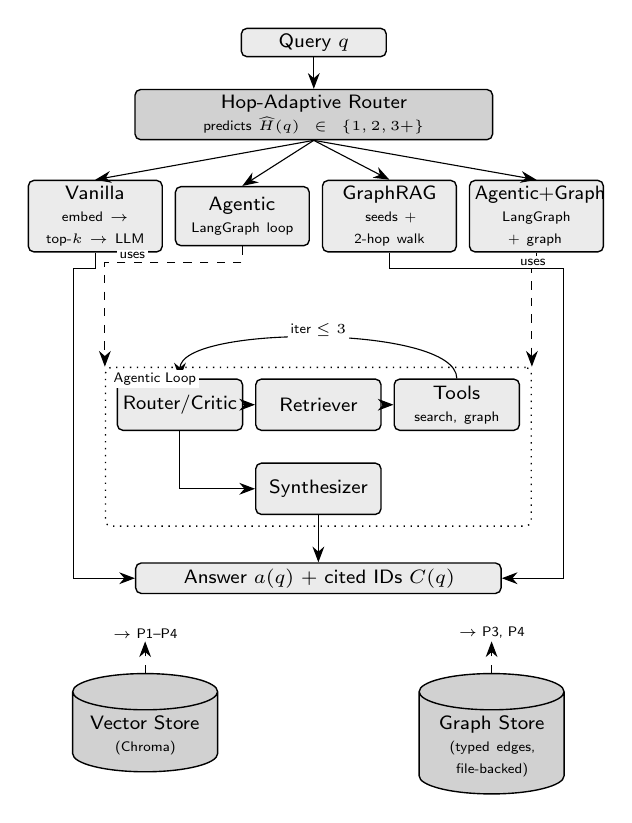
\begin{tikzpicture}[
  node distance=4mm,
  >={Stealth[length=2mm]},
  every node/.style={font=\sffamily\scriptsize}
]
\tikzset{
  box/.style    ={draw=black, line width=0.5pt, rounded corners=2pt,
                  align=center, inner sep=2pt},
  light/.style  ={box, fill=black!8},
  mid/.style    ={box, fill=black!18},
  pipe/.style   ={light, text width=1.55cm, minimum width=1.7cm,
                  minimum height=7.5mm},
  lp/.style     ={light, text width=1.45cm, minimum width=1.55cm,
                  minimum height=6.5mm},
  store/.style  ={cylinder, shape border rotate=90, aspect=0.25,
                  draw=black, line width=0.5pt, fill=black!18,
                  align=center, inner sep=2pt,
                  text width=1.7cm, minimum height=7mm},
  arr/.style    ={->, line width=0.4pt},
  darr/.style   ={arr, dashed},
  lab/.style    ={font=\sffamily\tiny, fill=white, inner sep=1pt},
  group/.style  ={draw=black, line width=0.5pt, rounded corners=2pt,
                  dotted, inner sep=4pt}
}

%% ----- Top: Query, Router -----
\node[light, text width=1.7cm] (q) at (0,0) {Query $q$};
\node[mid, below=4mm of q, text width=4.4cm] (router)
  {Hop-Adaptive Router\\{\tiny predicts $\widehat{H}(q) \in \{1, 2, 3{+}\}$}};
\draw[arr] (q) -- (router);

%% ----- Pipelines (centered at x=0) -----
\node[pipe, below=5mm of router, xshift=-2.775cm] (p1)
  {Vanilla\\{\tiny embed $\to$ top-$k$ $\to$ LLM}};
\node[pipe, right=1.5mm of p1] (p2)
  {Agentic\\{\tiny LangGraph loop}};
\node[pipe, right=1.5mm of p2] (p3)
  {GraphRAG\\{\tiny seeds + 2-hop walk}};
\node[pipe, right=1.5mm of p3] (p4)
  {Agentic+Graph\\{\tiny LangGraph + graph}};
\foreach \i in {1,2,3,4}
  \draw[arr] (router.south) -- (p\i.north);

%% ----- Agentic Loop subgraph (centered below pipelines) -----
\node[lp] (critic) at (-1.7,-4.6) {Router/Critic};
\node[lp, right=1.5mm of critic] (retr)  {Retriever};
\node[lp, right=1.5mm of retr]   (tools) {Tools\\{\tiny search, graph}};
\node[lp, below=4mm of retr]     (synth) {Synthesizer};

\draw[arr] (critic) -- (retr);
\draw[arr] (retr)   -- (tools);
\draw[arr] (tools.north) to[out=90,in=90,looseness=0.5]
  node[lab, midway, yshift=1mm] {iter $\le 3$} (critic.north);
\draw[arr] (critic.south) |- (synth.west);

\begin{scope}[on background layer]
  \node[group, fit=(critic)(retr)(tools)(synth)] (loop) {};
\end{scope}
\node[lab, anchor=north west]
  at ([xshift=2pt,yshift=-1pt]loop.north west) {Agentic Loop};

%% ----- P2, P4 -> Loop (dashed "uses"; right-angle elbows) -----
\draw[darr] (p2.south) -- ++(0,-2mm) -| (loop.north west)
  node[lab, pos=0.4, above] {uses};
\draw[darr] (p4.south) -- ++(0,-2mm) -| (loop.north east)
  node[lab, pos=0.4, above] {uses};

%% ----- Output -----
\node[light, below=6mm of synth, text width=4.5cm] (out)
  {Answer $a(q)$ + cited IDs $C(q)$};
\draw[arr] (synth.south) -- (out.north);

%% ----- P1, P3 -> Output (bypass loop on the sides) -----
\draw[arr] (p1.south) -- ++(0,-2mm) -|
  ([xshift=-4mm]loop.south west) |- (out.west);
\draw[arr] (p3.south) -- ++(0,-2mm) -|
  ([xshift=4mm]loop.south east)  |- (out.east);

%% ----- Data stores at the bottom; consolidated arrows -----
\node[store, below=10mm of out, xshift=-22mm] (s1)
  {Vector Store\\{\tiny (Chroma)}};
\node[store, below=10mm of out, xshift=22mm]  (s2)
  {Graph Store\\{\tiny (typed edges, file-backed)}};

\draw[darr] (s1.north) -- ++(0,4mm)
  node[lab, anchor=south] {$\to$ P1--P4};
\draw[darr] (s2.north) -- ++(0,4mm)
  node[lab, anchor=south] {$\to$ P3, P4};

\end{tikzpicture}
}%
  \caption{The five pipelines and their shared components. Vanilla and
    GraphRAG make a single synthesis call. Agentic and Agentic+Graph run
    a router, retriever, tool, and critic loop for at most three
    iterations before synthesis. The adaptive pipeline (rule-based V1 or
    learned V2) selects one of the four base pipelines per query.}
  \label{fig:architecture}
\end{figure}

\subsection{Pipelines}
\label{sec:pipelines}
All pipelines share the embedder, a ChromaDB vector store, a file-backed
typed-edge graph, the GPT-5.4 generator, and a grounded synthesis
prompt, so they differ only in how they retrieve
(Fig.~\ref{fig:architecture}).
\textbf{(i)~Vanilla} retrieves the top 10 chunks by dense similarity,
passes the top 5 to the synthesizer, and makes one synthesis call.
\textbf{(ii)~Agentic} is a LangGraph~\cite{langgraph_software} loop of
router, retriever, and critic with a single \texttt{search\_documents}
tool and at most three iterations.
\textbf{(iii)~GraphRAG} takes 8 vector seeds, walks up to two hops in
the typed graph (at most 30 nodes), and passes at most 15 chunks to one
synthesis call. It is a local-walk retriever in the GraphRAG family
rather than the community-summarisation system of Edge
et al.~\cite{graphrag2024}; we use ``GraphRAG'' as the family name.
\textbf{(iv)~Agentic+Graph} adds a typed \texttt{graph\_lookup} tool to
(ii). \textbf{(v)~Adaptive} chooses among (i) to (iv) for each query. We
evaluate a rule-based router (V1) and a learned router (V2), an
out-of-fold logistic regression over 11 text features and 3
principal components of the query embedding that sends each predicted
hop class to its empirically best pipeline.

\subsection{Experimental Factors}
\label{sec:axes}
\textbf{Embedder.} We use three models from three vendors at three
dimensionalities: e5-small (384 dimensions), OpenAI
text-embedding-3-small (1536), and BAAI bge-m3 (1024). The vector index is rebuilt per embedder; the graph is shared.
\textbf{Traversal.} Besides the bounded undirected walk (at most two
hops, at most 30 nodes), we run personalized PageRank from the same
vector seeds. It is unbounded in radius and ranks nodes by random-walk
mass, and all other settings are held fixed.
\textbf{Corpus.} The main corpus is a synthetic DO-178C-style
collection of 1{,}132 aerospace requirements in 30 modules (17 to 76
requirements per module; median length 59 tokens, 90th percentile 103).
GPT-5.4 generated it from a hand-authored module taxonomy, and we
release it with its link annotations. Retrieval traverses five
traceability edge types (\textit{derives\_from}, \textit{satisfies},
\textit{references}, \textit{verifies}, and \textit{refines}); we exclude
system-engineering edges such as allocation, which do not help
retrieval. Two Wikipedia corpora test transfer: 200 MuSiQue~\cite{musique2022}
questions (67, 67, and 66 of two, three, and four hops, mapped to our
three strata, with \textit{REFERENCES} edges between consecutive
supporting paragraphs) and 200 2WikiMultihopQA~\cite{twowiki2020}
questions, stratified by reasoning type: \textit{comparison} questions are one-hop,
\textit{compositional} and \textit{inference} questions are two-hop, and
\textit{bridge\_comparison} questions are three-or-more-hop.
\textbf{Judge.} Faithfulness is judged by GPT-5.4, GPT-4.1, and
Gemini 3.7-flash (Section~\ref{sec:experiments}).

\subsection{Queries and Gold Evidence}
\label{sec:queries}
We build the DO-178C queries from the graph rather than by free-form
prompting. We sample directed chains of one, two, and three to four
requirement links over the five edge types and prompt GPT-5.4 to phrase
one natural-language question that the chain answers. The nodes of the
chain form the gold evidence, so the gold set grows with the stratum
(on average 2.00, 3.00, and 4.68 IDs). This yields 296 queries (100,
99, and 97 per stratum), of which 85\% cross module boundaries; 497 of
the 655 chain edges are \textit{references} links. The gold sets are structural rather than human-annotated: a sampled
chain is a supporting path by construction, but we do not verify that
no other path answers the question. Citation recall is therefore exact
and precision conservative, equally for all pipelines.

\subsection{Metrics}
\label{sec:metrics}
We report citation precision, recall, and $F_1$ against the gold ID
sets, following ALCE~\cite{alce2023}. Cited IDs are parsed from the
answer text with a parser anchored to the corpus vocabulary, which
matches exact IDs and prefers the longest match. Hallucinated IDs that
reuse a real module prefix count against precision, and incidental
tokens such as SHA-256 or DO-254 are ignored. We report separately the context precision (the gold fraction of the
chunks handed to the synthesizer) and the retrieval recall, since
conflating context and citations changes which architecture appears to
win (Section~\ref{sec:c2}).

Each faithfulness judgment is a binary verdict, returned as strict JSON,
on whether the answer is supported by the retrieved context. For
agreement we report Cohen's $\kappa$, Gwet's
AC1~\cite{gwet2008,feinstein1990}, raw agreement, and an exact McNemar
test. For each faithfulness cell we report a Wilson 95\% confidence
interval and a Cochran--Armitage test for trend over hop depth. Three
same-judge controls (test--retest, embedder swap, and re-judging after
eleven weeks) use a paired subset of 300 tuples
(Section~\ref{sec:c4}).

\section{Experimental Setup}
\label{sec:experiments}

\noindent\textbf{Runs.} On DO-178C, we run 5 pipelines $\times$ 296 queries
$\times$ 3 seeds, giving 4{,}440 runs under each of two embedders
(e5-small, which we call \emph{v2}, and text-embedding-3-small,
\emph{v3}). We add 1{,}480 runs at one seed under bge-m3 (\emph{v4})
and a 296-run personalized PageRank arm under the v3 embedder. On
MuSiQue, we run vanilla, GraphRAG, and agentic+graph on 200 queries at
one seed (600 runs, v3 embedder), since RQ2 needs only these three, and
extend the GraphRAG arm to three seeds to match DO-178C's per-stratum
sample. On the same queries we add 400 runs for two mitigations and a
200-run GraphRAG control with distractor edges (Section~\ref{sec:c1}).
On 2WikiMultihopQA, we run vanilla and GraphRAG on 200 queries at three
seeds (1{,}200 runs, v3 embedder).

\noindent\textbf{Faithfulness judging.} On DO-178C, GPT-5.4 and GPT-4.1 judge
two disjoint stratified batches of 300 rows each (60 per pipeline;
seeds 42 and 43), the second eleven weeks after the first. Each batch is
fixed to the same 300 (query, pipeline, repeat) tuples across
embedders, so embedder differences are computed on identical items, and
batches judged on different dates are never pooled. In a later pass, GPT-4.1
and Gemini 3.7-flash judge every row of the DO-178C matrices and of the
Wikipedia corpora. Gemini judged four days after GPT-4.1 on DO-178C and
one day after it on the Wikipedia corpora, in both cases on the same
stored answer and context strings, so the pairing is exact at the row
level. Two same-input
controls re-judge 300 v2 tuples with GPT-5.4, once on the same day
(test--retest) and once eleven weeks later. A generator-swap control
re-synthesizes 332 v3 rows with GPT-4.1 on frozen retrievals and judges
them with both judges.

\noindent\textbf{Statistical protocol.} We compute 95\% BCa bootstrap
intervals~\cite{du2025bootstrap} with 1{,}000 resamples paired at the
query level, Wilcoxon signed-rank tests with Holm correction over the
30 contrasts of pipeline pair and stratum~\cite{bergkirkpatrick2012,koehn2004},
and Cliff's $\delta$, which we treat as negligible below 0.147. We call
two pipelines significantly different only when the BCa interval
excludes zero, the Holm-adjusted $p$ is below 0.05, and
$|\delta| \ge 0.147$. Tests pool the three seeds; we report the spread across seeds
separately (Section~\ref{sec:c1}).

\noindent\textbf{Reproducibility.} The original graph store was populated
before this study and contains edges beyond those annotated in the
released corpus. Loading the release with our ETL recovers 91.0\% of
the edges and 82.8\% of the chains behind our queries. Every gold set is
nevertheless exact, since the query manifest is released with its full
chains. The v2 and v3 graph arms walked the original store, while
the bge-m3 matrix and the PageRank arm walked a file-backed store built
from the released annotations, which is also what a reproduction uses.
To check that the change of graph does not drive our comparisons, we
rebuilt every v3 GraphRAG context on the file-backed store without
generation. The vector seeds are identical for 295 of the 296 queries,
the two contexts have a Jaccard overlap of 0.89, and context precision
(0.131 against 0.129) and retrieval recall (0.720 against 0.724) differ
by at most 0.01 in every stratum. We did not regenerate answers on the
new store, so the citation side of this check is untested.
We use the Azure snapshots \texttt{gpt-5.4-}\allowbreak\texttt{2026-03-05}
(generator and judge) and \texttt{gpt-4.1-2025-04-14} (judge) in
reasoning mode, with a completion cap of 8{,}192 tokens. The MuSiQue
subgraph (3{,}996 paragraph chunks and 399 \textit{REFERENCES} edges) is
built deterministically from the \texttt{dgslibisey} mirror (validation
split, seed 20260511), and the 2WikiMultihopQA subgraph (2{,}000 chunks
and 332 edges) from the \texttt{voidful} mirror (seed 20260816) by the
same procedure.

\section{Results}
\label{sec:results}

\begin{table*}[t]
  \centering
  \caption{Citation $F_1$ by hop stratum in four settings. v2 and v3: DO-178C with the e5-small and text-embedding-3-small embedders (4{,}440 runs each). MuSiQue: 200 queries with the v3 embedder (600 runs; vanilla, agentic+graph, and GraphRAG only). 2Wiki: 200 2WikiMultihopQA queries at three seeds (1{,}200 runs; vanilla and GraphRAG only). Bold marks the best pipeline per setting and stratum.}
  \label{tab:dominance}
  \footnotesize\setlength{\tabcolsep}{3pt}
  \resizebox{\textwidth}{!}{%
  \begin{tabular}{l ccc | ccc | ccc | ccc}
    \toprule
     & \multicolumn{3}{c|}{v2 main (local)} & \multicolumn{3}{c|}{v3 main (Azure)} & \multicolumn{3}{c|}{MuSiQue (Azure)} & \multicolumn{3}{c}{2Wiki (Azure)} \\
    System & 1h & 2h & 3+h & 1h & 2h & 3+h & 1h & 2h & 3+h & 1h & 2h & 3+h \\
    \midrule
    vanilla & \textbf{.757} & .712 & .089 & \textbf{.756} & .689 & .195 & .742 & .415 & .277 & \textbf{.990} & .778 & .678 \\
    agentic & .541 & .414 & .175 & .533 & .430 & .203 & --- & --- & --- & --- & --- & --- \\
    agentic-graph & .566 & .415 & \textbf{.219} & .547 & .421 & .251 & .457 & .296 & .249 & --- & --- & --- \\
    graphrag & .751 & \textbf{.720} & .172 & .745 & \textbf{.707} & .253 & \textbf{.841} & \textbf{.632} & \textbf{.463} & .969 & \textbf{.946} & \textbf{.938} \\
    adaptive & .630 & .499 & .181 & .651 & .492 & \textbf{.254} & --- & --- & --- & --- & --- & --- \\
    \bottomrule
  \end{tabular}}
\end{table*}


\begin{figure}[t!]
  \centering
  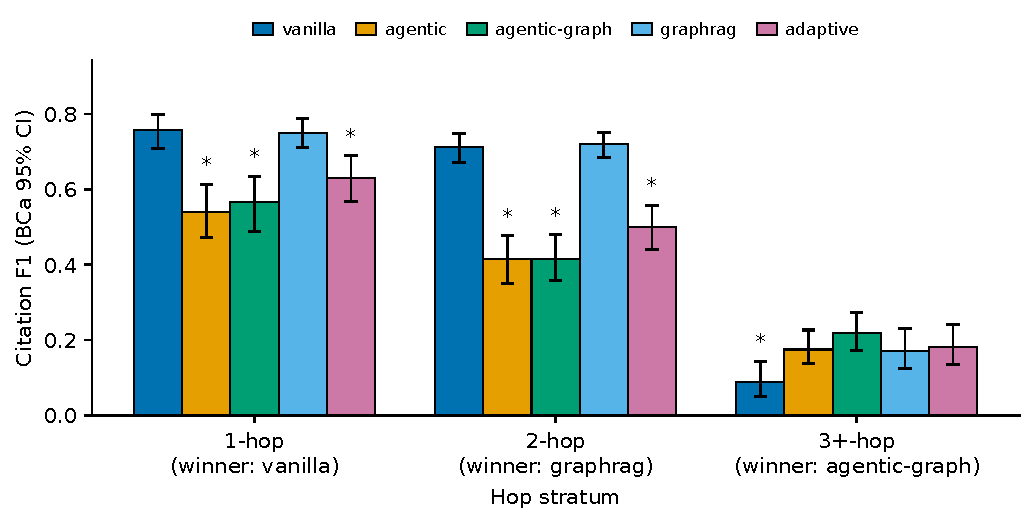
\includegraphics[width=0.55\textwidth]{figures/fig1_per_stratum_f1.pdf}
  \caption{Citation $F_1$ by hop stratum on the v2 matrix (DO-178C,
    e5-small), with 95\% BCa intervals. An asterisk marks a pipeline that
    differs significantly from the best pipeline in its stratum (Holm-adjusted
    Wilcoxon $p < 0.05$ and $|\delta| \ge 0.147$).}
  \label{fig:perstratum}
\end{figure}

\subsection{Citation Quality by Hop Depth (RQ1)}
\label{sec:c1}
Table~\ref{tab:dominance} reports citation $F_1$ by stratum in four
settings. On DO-178C, vanilla and GraphRAG are statistically tied on
one- and two-hop queries (Wilcoxon $p = 0.12$ and $0.65$ under the v2
embedder, with negligible $\delta$), and the agentic loop costs 0.19 to
0.30 $F_1$ on these strata. On queries of three or more hops the
ordering reverses. Vanilla falls to last place, and the pipelines that
use the graph lead; under the v2 embedder agentic+graph reaches 0.219
against 0.089 for vanilla (Holm $p < 10^{-6}$). Under the v3 embedder the ordering is the same, but no pair at this depth passes the joint criterion. Under bge-m3 the pattern recurs (Table~\ref{tab:embedders}):
vanilla is last at three or more
hops under all three embedders, and under bge-m3 both graph pipelines
outperform it by 0.100 and 0.091 (Holm $p = 2.1 \times 10^{-4}$ and
$1.4 \times 10^{-3}$), while the one- and two-hop contrasts remain
negligible.

On MuSiQue, GraphRAG is best in every stratum ($F_1$ of 0.841, 0.632,
and 0.463), with $p \le 5.1 \times 10^{-4}$ and $\delta$ between 0.27
and 0.43 against vanilla. Because the MuSiQue \textit{REFERENCES} edges
connect only gold paragraphs, we also ran GraphRAG on a graph with
additional edges between consecutive distractor paragraphs. GraphRAG
then loses 0.02, 0.05, and 0.09 $F_1$ per stratum and still outperforms
vanilla in every stratum ($p \le 0.014$), so its advantage on MuSiQue
does not depend on gold-only edges. On 2WikiMultihopQA, the two
pipelines are tied on one-hop queries ($p = 0.15$), and GraphRAG leads
on two-hop and deeper queries by 0.168 and 0.260 ($\delta = 0.48$ and
0.87). This is the DO-178C crossover again, on a graph we did not build.

Seed variation is small by comparison. The mean $F_1$ of each pipeline
changes by at most 0.031 between seeds,
every significant ordering holds in each seed separately, and the only
changes in rank occur between vanilla and GraphRAG on one- and two-hop
queries, which we already report as ties. Regarding RQ1, the best
pipeline depends on hop depth and on the corpus, but not on the embedder
or the seed.

\begin{table}[t]
  \centering
  \caption{Citation $F_1$ by hop stratum on DO-178C under three embedders from three vendors (e5-small, 384 dimensions; text-embedding-3-small, 1536; bge-m3, 1024). Bold marks the best pipeline per embedder and stratum.}
  \label{tab:embedders}
  \small
  \setlength{\tabcolsep}{4pt}
    \begin{tabular}{l rrr rrr rrr}
    \toprule
    & \multicolumn{3}{c}{e5-small (384d)} & \multicolumn{3}{c}{3-small (1536d)} & \multicolumn{3}{c}{bge-m3 (1024d)} \\
    \cmidrule(lr){2-4}\cmidrule(lr){5-7}\cmidrule(lr){8-10}
    System & 1h & 2h & 3+h & 1h & 2h & 3+h & 1h & 2h & 3+h \\
    \midrule
    vanilla       & \textbf{.757} & .712 & .089 & \textbf{.756} & .689 & .195 & \textbf{.769} & .691 & .114 \\
    agentic       & .541 & .414 & .175 & .533 & .430 & .203 & .548 & .404 & .156 \\
    agentic-graph & .566 & .415 & \textbf{.219} & .547 & .421 & .251 & .546 & .431 & .206 \\
    graphrag      & .751 & \textbf{.720} & .172 & .745 & \textbf{.707} & .253 & .742 & \textbf{.728} & \textbf{.214} \\
    adaptive      & .630 & .499 & .181 & .651 & .492 & \textbf{.254} & .672 & .478 & .202 \\
    \bottomrule
  \end{tabular}
\end{table}


\begin{table}[t]
  \centering
  \caption{Context and citation precision of GraphRAG in six settings. Slots: chunks passed to the synthesizer. IDs: IDs cited in the answer. Gain: citation precision divided by context precision.}
  \label{tab:pathology}
  \small
  \setlength{\tabcolsep}{4pt}
  \begin{tabular}{l rr rr r}
    \toprule
    & \multicolumn{2}{c}{\textit{retrieved context}} & \multicolumn{2}{c}{\textit{answer citations}} & \\
    \cmidrule(lr){2-3}\cmidrule(lr){4-5}
    Setting & slots & prec. & IDs & prec. & gain \\
    \midrule
    DO-178C, e5-small     & 14.9 & 0.120 & 4.9 & 0.480 & 4.0$\times$ \\
    DO-178C, 3-small      & 14.9 & 0.129 & 5.0 & 0.493 & 3.8$\times$ \\
    DO-178C, bge-m3       & 14.8 & 0.121 & 4.7 & 0.490 & 4.1$\times$ \\
    DO-178C, PPR walk     & 14.9 & 0.131 & 4.9 & 0.509 & 3.9$\times$ \\
    MuSiQue               & 11.2 & 0.227 & 3.4 & 0.654 & 2.9$\times$ \\
    2WikiMultihopQA       & 11.4 & 0.230 & 2.5 & 0.975 & 4.2$\times$ \\
    \bottomrule
  \end{tabular}
\end{table}


\begin{figure}[t!]
  \centering
  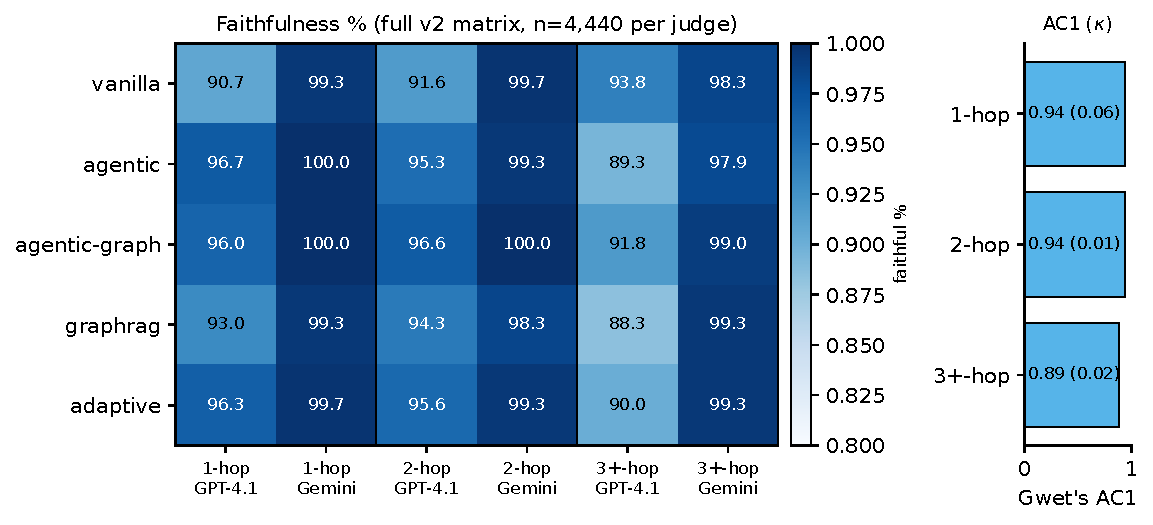
\includegraphics[width=0.8\textwidth]{figures/fig2_faithfulness_heatmap.pdf}
  \caption{Faithfulness on the full v2 matrix (DO-178C, e5-small; 4{,}440
    rows, about 300 per cell), judged by GPT-4.1 and Gemini 3.7-flash on
    the same rows. Left: percentage of answers judged faithful. Right:
    Gwet's AC1 between the two judges per stratum, with Cohen's $\kappa$
    in parentheses. The colour scale starts at 80\%.}
  \label{fig:faithheatmap}
\end{figure}

\subsection{Context Versus Answer Citations (RQ2)}
\label{sec:c2}
Table~\ref{tab:pathology} reports the same measurement in six settings,
covering three embedders, three corpora, and two traversals. GraphRAG's
walk fills 11 to 15 context slots at a context precision of 0.12 to
0.23, so four or five of every six chunks it retrieves are not gold. The
synthesizer then cites only 2.5 to 5.0 IDs per answer, at a citation
precision of 0.48 to 0.98. In every setting, the precision of the
citations is 2.9 to 4.2 times that of the context. The $F_1$ advantage
of GraphRAG is therefore a recall effect: the walk retrieves gold chunks
that dense retrieval misses, and the synthesizer does not cite most of
the irrelevant chunks that come with them.

An evaluation that scores the retrieved set as the attribution set, as
some GraphRAG comparisons do, sees only the first step and reaches the
opposite ranking. By context precision, GraphRAG
is below the vanilla baseline in every setting (0.12 to 0.23, against
0.27 to 0.37 for vanilla). By citation $F_1$, it is the best pipeline in
every setting, with scores of 0.551, 0.571, 0.565, 0.585, 0.646, and
0.951 in the row order of Table~\ref{tab:pathology}. 

Two controls test whether this depends on our design. The first
replaces the two-hop walk with personalized PageRank over the same
graph. Context
precision is 0.131 with PageRank and 0.129 with the original walk (0.131
for the walk rebuilt on the same file-backed graph;
Section~\ref{sec:experiments}). The precision gain from context to
citations is 3.9 and 3.8 times, and the difference in citation $F_1$ is
0.016 with $\delta = 0.036$, which our criterion treats as negligible.
The second control applies two mitigations on MuSiQue. Reranking the
walked neighbours by similarity to the query and keeping the top five
changes little (context precision from 0.227 to 0.232, citation $F_1$
$+0.010$, $p = 0.34$). Reducing the traversal budget from 30 to 10 nodes
and the context from 15 to 8 chunks lowers citation $F_1$ by 0.126
($p = 2.6 \times 10^{-11}$) and also lowers context precision, to 0.194.
Both outcomes fit a synthesizer that already filters: an upstream
filter adds little, and a smaller budget removes the recall the
advantage depends on. Regarding RQ2, the comparison
reverses with the measurement point in all six settings.

\subsection{Faithfulness and Hop Depth (RQ3)}
\label{sec:c3}
On 300-row judged subsets, faithfulness declines with hop depth on
DO-178C but not on the Wikipedia chains. This difference disappears at
adequate power. The MuSiQue arm had 67 rows per
stratum. Its drop from one-hop to three-or-more-hop queries (9.2
percentage points) was larger than the 4.7-point drop that is
significant on DO-178C, but detecting it with 80\% power requires about
210 rows per cell. With three seeds ($n = 600$), the decline is
significant under both judges, from 0.930 to 0.876 to 0.823 under GPT-4.1
($p = 1.1 \times 10^{-3}$) and from 0.955 to 0.945 to 0.869 under Gemini
($p = 1.2 \times 10^{-3}$). On 2WikiMultihopQA, judged in full
($n = 1{,}200$), faithfulness also declines ($p = 5.0 \times 10^{-2}$ and
$4.8 \times 10^{-6}$). The decline therefore replicates on all three
corpora under two vendors.

What distinguishes the pipelines is whether they expand the context.
Vanilla retrieves a fixed top five and adds nothing, and under GPT-4.1
it shows no significant drop from one-hop to three-or-more-hop queries.
Its change is $-1.5$ points on DO-178C ($n = 2{,}072$; $p = 0.16$, 0.99,
and 0.76 for the three embedders) and $+1.1$ points on 2WikiMultihopQA
($p = 0.66$). The four expanding pipelines drop by 6.3 and 6.7 points on
the same corpora (Fig.~\ref{fig:faithheatmap}). A logistic regression
of faithfulness on hop depth, an expansion indicator, and their
interaction turns this contrast into a single test. The interaction is
negative and significant on the pooled DO-178C matrix ($b = -0.599$,
$p = 1.0 \times 10^{-7}$, $n = 10{,}360$), and negative but not
significant on 2WikiMultihopQA ($b = -0.286$, $p = 0.27$), whose arm is
one twentieth the size.

Under Gemini the ordering is the same, but the test does not resolve.
Near the ceiling, vanilla itself shows a slope ($b = -0.729$,
$p = 0.012$), and the interaction cannot be separated from it
($p = 0.11$). The expanding pipelines still drop more than vanilla (2.8
against 1.5 points on DO-178C, 12.7 against 7.7 on 2WikiMultihopQA). A lenient judge preserves the ranking but not the power to test it
(Section~\ref{sec:c4}). Not every expanding pipeline declines in every cell: GraphRAG is
marginal under bge-m3 ($p = 0.065$), and the agentic pipelines decline
in four of six embedder and pipeline combinations. We have not re-run the GPT-5.4
judge at this sample size. Regarding RQ3, faithfulness declines with
hop depth on every corpus, and the decline is steeper for pipelines
that expand their context.

\begin{table}[t]
  \centering
  \caption{Judge agreement. Top: the same judge re-judging identical answer and context strings, so only the date differs. Middle: the same judge after an embedder swap changes the input. Bottom: GPT-4.1 against Gemini 3.7-flash on identical rows; the last column gives the fraction judged faithful by each.}
  \label{tab:judges}
  \small
  \setlength{\tabcolsep}{4pt}
    \begin{tabular}{l rrrr}
    \toprule
    \multicolumn{5}{l}{\textit{Same judge, frozen input (answer + context identical)}} \\
    \midrule
    GPT-5.4, re-judged same day & \multicolumn{4}{r}{$\kappa = 0.764$, raw agr.\ 0.88} \\
    GPT-5.4, re-judged 11 wk later & \multicolumn{4}{r}{$\kappa = 0.138$, raw agr.\ 0.56} \\
    GPT-4.1, re-judged 11 wk later & \multicolumn{4}{r}{$\kappa = -0.05\,/\,-0.00$ (v2/v3), raw agr.\ 0.48\,/\,0.51} \\
    GPT-4.1, full matrix vs.\ May & \multicolumn{4}{r}{$\kappa = -0.046$, raw agr.\ 0.48, $+43$\,pp} \\
    \midrule
    \multicolumn{5}{l}{\textit{Same judge, input changed by embedder swap}} \\
    \midrule
    GPT-5.4 (v2 vs v3) & \multicolumn{4}{r}{$\kappa = 0.137$, raw agr.\ 0.59} \\
    GPT-4.1 (v2 vs v3) & \multicolumn{4}{r}{$\kappa = 0.480$, raw agr.\ 0.74} \\
    \midrule
    \multicolumn{5}{l}{\textit{Cross-vendor, same rows (Gemini 3.7-flash vs.\ GPT-4.1)}} \\
    \midrule
    \textit{Setting} & raw & $\kappa$ & AC1 & faithful (G\,/\,4.1) \\
    \midrule
    DO-178C e5-small ($n{=}4{,}440$) & 0.929 & 0.029 & 0.923 & 0.993 / 0.933 \\
    DO-178C 3-small ($n{=}4{,}440$)  & 0.913 & 0.125 & 0.903 & 0.980 / 0.917 \\
    DO-178C bge-m3 ($n{=}1{,}480$)   & 0.939 & 0.047 & 0.935 & 0.991 / 0.945 \\
    DO-178C PPR walk ($n{=}296$)     & 0.926 & 0.058 & 0.919 & 0.983 / 0.936 \\
    MuSiQue, 3 seeds ($n{=}600$)     & 0.850 & 0.172 & 0.817 & 0.923 / 0.877 \\
    MuSiQue rerank ($n{=}200$)       & 0.820 & 0.171 & 0.772 & 0.935 / 0.825 \\
    MuSiQue budget cap ($n{=}200$)   & 0.875 & 0.419 & 0.841 & 0.875 / 0.880 \\
    2WikiMultihopQA ($n{=}1{,}200$)  & 0.899 & 0.435 & 0.877 & 0.888 / 0.914 \\
    \bottomrule
  \end{tabular}
\end{table}


\subsection{Judge Stability (RQ4)}
\label{sec:c4}
Table~\ref{tab:judges} separates instability on fixed inputs from
instability after the retrieval state changes.
\textit{Fixed inputs.} Re-judging the same 300 stored answer and
context pairs gives GPT-5.4 a self-agreement of $\kappa = 0.76$ (raw
agreement 0.88) on the same day, but only $\kappa = 0.14$ (raw agreement
0.56) eleven weeks later, with 15 points more answers judged faithful.
This rejects a stationary judge (binomial $p < 10^{-44}$). GPT-4.1 on the same tuples agrees with its own earlier
verdicts only at chance level ($\kappa = -0.05$ and $-0.00$ for v2 and
v3) and judges 41 points more answers faithful. With fixed inputs, this is drift of the judge alone.
\textit{Changed retrieval state.} After an embedder swap, which
changes the context and the answer for 94\% of the tuples, GPT-5.4
changes 41\% of its verdicts ($\kappa = 0.137$) and GPT-4.1 changes 26\%
($\kappa = 0.48$). The judge that is more stable under the embedder
swap is thus the less stable over time.
\textit{Across vendors.} On the same rows, Gemini 3.7-flash is much
more lenient than GPT-4.1 on all four DO-178C settings (0.98 to 0.99
against 0.92 to 0.95 faithful; McNemar $p < 10^{-9}$). They are indistinguishable on the budget-capped MuSiQue arm (0.875 against 0.880,
$p = 1.00$), and Gemini is stricter on 2WikiMultihopQA (0.888 against
0.914, $p = 6.2 \times 10^{-3}$). Strictness is therefore a property of
the judge and corpus together, and a calibration offset measured on one
corpus cannot be reused on another. The same eight
settings show the prevalence paradox~\cite{feinstein1990} within one
pair of judges. Raw agreement ranges only from 0.82 to 0.94, and Gwet's
AC1 follows it (0.77 to 0.94), whereas $\kappa$ ranges from 0.03 to
0.44, ordered almost exactly by the distance of faithfulness from the
ceiling. On 2WikiMultihopQA the two judges agree less often than on
DO-178C (0.899 against 0.93), yet their $\kappa$ is fifteen times
higher (0.435 against 0.029). Leniency and trend are nevertheless
separate properties. Although Gemini is near the ceiling on DO-178C, it
reproduces the decline with hop depth on both DO-178C matrices
($p = 4.3 \times 10^{-3}$ and $p < 10^{-16}$) and on both Wikipedia
corpora. The ordering a judge induces replicates across vendors, while
its strictness does not.
\textit{Between judges.} Inter-judge agreement halves under the embedder swap ($\kappa$ from
0.30 to 0.17; McNemar $p < 0.001$), and on the 300-row MuSiQue batch
GPT-5.4 and GPT-4.1 agreed only at chance (raw agreement 0.48, AC1
0.08), a real disagreement rather than a prevalence effect. We therefore
re-judged the full matrix within one judging period
(Section~\ref{sec:c3}), and no comparison we report spans judging
dates. Regarding RQ4, judges are not stable over
time, across retrieval states, or across vendors, although the hop-wise
ordering they induce is.

\section{Discussion}
\label{sec:discussion}

\paragraph{Why expansion lowers faithfulness.}
The synthesizer leaves most irrelevant chunks out of its citations
(Section~\ref{sec:c2}), but they can still influence the answer. Because faithfulness is judged
against the full retrieved context, every chunk the walk adds is one
more chunk the answer can be judged unfaithful to. This mechanism does not depend on what the edges connect, consistent
with the decline on both typed DO-178C links and Wikipedia paragraph
links. The cost appears to scale with the number of added chunks
rather than with their relevance, since reranking them by relevance
changes nothing (Section~\ref{sec:c2}).

\paragraph{Implications for LLM judges.}
Since judges change with the retrieval state and the date
(Section~\ref{sec:c4}), single-judge comparisons of retrieval modules
are conditional on both, and ensembles help only partially. At a
minimum, faithfulness should be compared on paired tuples under a fixed
embedder and judged within one period.

\paragraph{Threats to validity.}
\emph{Construct validity.} Citation $F_1$ does not measure the quality
of the reasoning, so we pair it with faithfulness judgments, which are
themselves subject to bias~\cite{selfpref_bias2024,wallat2024}. We
quantify this bias directly (Section~\ref{sec:c4}) and use a third
judge from a different vendor on every matrix.
\emph{External validity.} The DO-178C corpus is a single synthetic
dataset, generated by the same model family that answers and judges,
and its absolute $F_1$ levels may not transfer to other regulated
domains. When GPT-4.1 re-synthesizes 332 answers on frozen retrievals, the
pipeline ordering and the faithfulness decline both hold, so neither
result is specific to GPT-5.4. The corpus, however, is still written by that family. The two Wikipedia
corpora, judged in full by two vendors, are our main check of external
validity; both reproduce the RQ1 crossover, although only DO-178C
includes all five pipelines. Our GraphRAG pipeline is one
local-walk implementation. Replacing the walk with personalized
PageRank leaves the RQ2 result unchanged, but a full third-party
GraphRAG system may flood or filter its context differently. The two
unsupervised mitigations we tried did not help, and a learned evidence
selector conditioned on the question remains to be tested.
\emph{Statistical conclusion validity.} Per-stratum samples for the citation metrics (97 to 100 queries on
DO-178C, 66 to 67 on Wikipedia) are at the lower end of BCa stability
under strong skew, but percentile intervals give the same conclusions. Faithfulness cells hold about 300 rows after full-matrix judging. The
hop-by-expansion interaction is significant on DO-178C, but on the much
smaller 2WikiMultihopQA arm we can report only its direction.

\paragraph{Artifact availability.}
The corpus with its link annotations, the query manifest with full
chains, the code, and every scored and judged CSV file are released
under CC-BY-4.0 \ifanonymous (links withheld for review)\else at
\url{https://huggingface.co/datasets/meftun/aerosys-requirements} and
\url{https://github.com/mftnakrsu/rag-vs-agentic}\fi. The Wikipedia
subsets are rebuilt by seeded scripts.

\section{Conclusion}
\label{sec:conclusion}
In this paper, we compared five RAG pipelines for multi-hop
requirements traceability while varying the embedder, corpus, graph
traversal, and judge. The citation measurement point reverses the
GraphRAG comparison in all six settings, the best pipeline per hop
depth is stable across embedders and seeds, and the faithfulness
decline follows context expansion on all three corpora. LLM judges
drift on identical inputs but agree on the hop-wise ordering. RAG
comparisons should therefore state their measurement point and report
results across these factors; testing a learned evidence selector and a
third-party GraphRAG system are natural next steps.


\bibliographystyle{splncs04}
\bibliography{refs}

\end{document}

\documentclass[runningheads]{llncs}

\usepackage[T1]{fontenc}
\usepackage{lmodern}
\usepackage{booktabs}
\usepackage{amsmath}
\usepackage{amssymb}
\usepackage{graphicx}
\usepackage{xcolor}
\usepackage{tikz}
\usetikzlibrary{positioning, arrows.meta, shapes.geometric,
                fit, backgrounds, calc}
\usepackage{cite}
\usepackage{microtype}
\usepackage[hidelinks]{hyperref}

\newif\ifanonymous
\ifdefined\arxiv \anonymousfalse \else \anonymoustrue \fi

%% acmart's accessibility description; LNCS has no equivalent.
\newcommand{\Description}[1]{}

\begin{document}

\title{A Multi-Axis Robustness Analysis of Retrieval-Augmented Generation
  for Multi-Hop Requirements Traceability}
\titlerunning{Multi-Axis Robustness of RAG for Requirements Traceability}

\ifanonymous
\author{Anonymous Author(s)}
\authorrunning{Anonymous}
\institute{Anonymous Institution}
\else
\author{Meftun Akarsu\inst{1} \and
  Burak \"Ozdemir\inst{1} \and
  Do\u{g}ancan B\"uy\"uk\c{c}olak\inst{1} \and
  Recep Kaan Karaman\inst{2}}
\authorrunning{M. Akarsu et al.}
\institute{Turkish Aerospace Industries, Ankara, T\"urkiye \and
  Technical University of Munich, Munich, Germany\\
  \email{kaan.karaman@tum.de}}
\fi

\maketitle

\begin{abstract}
Published comparisons of GraphRAG and vector RAG reach conflicting
verdicts, and each typically rests on a single corpus, embedder, and
judge. We hold five RAG pipelines fixed and vary the embedder, the
corpus (DO-178C requirements, MuSiQue, and 2WikiMultihopQA), the graph
traversal, and the faithfulness judge, over 13{,}456 generation runs
and more than 30{,}000 judgments. We find that the point at which
citation quality is measured decides the comparison. GraphRAG's graph
walk fills the context with mostly irrelevant chunks, at a precision of
0.12 to 0.23, while its synthesizer cites selectively. Scored on the
retrieved context, GraphRAG therefore ranks below the vanilla baseline
in all six settings we test; scored on the answer's citations, it ranks
first. The best pipeline at each hop depth is stable across embedders
and seeds. Faithfulness declines with hop depth on all three corpora
once the comparison is adequately powered, and the decline follows
context expansion: the one pipeline that does not expand its context
does not decline. LLM judges, in contrast, are unstable. On identical
inputs re-judged eleven weeks later, self-agreement falls to
$\kappa \le 0.14$, and two vendors reverse which of them is stricter
between corpora. We recommend that RAG architecture comparisons report
the citation measurement point and be repeated across these factors.

\keywords{Retrieval-augmented generation \and GraphRAG \and Requirements traceability \and Multi-hop QA \and LLM-as-judge \and Evaluation methodology}
\end{abstract}

\section{Introduction}
\label{sec:intro}

Software traceability is the ability to relate each requirement to the
artifacts it derives from, satisfies, and is verified by. For airborne
software, DO-178C makes this relation a certification objective, and
certification authorities increasingly expect trace chains to be
auditable across two or more hops~\cite{do178c,arp4754a,easa2025npa,faa2024airoadmap}.
Because requirements management tools record these links explicitly, a
requirements corpus is also a typed link graph, and answering a
traceability question over it is a retrieval problem over both text and
graph.

Retrieval-augmented generation (RAG) is a natural fit for this task,
but published comparisons of RAG architectures disagree. Microsoft
GraphRAG~\cite{graphrag2024} exploits graph structure, yet loses to
vector RAG on detailed queries in recent
benchmarks~\cite{ragvsgraphrag2025,graphragbench2026}.
Adaptive-RAG~\cite{adaptiverag2024} routes queries by predicted
complexity but does not consider hop distance, and traceability systems
such as LiSSA~\cite{lissa2025} and TVR~\cite{niu_tvr2025} do not reason
over typed graphs. Each of these evaluations reports which architecture
wins in one setting, usually with one corpus, one embedder, and one
judge. They do not explain why the verdict changes when the setting
changes.

In this paper, we hold a matrix of five pipelines fixed (vanilla,
agentic, agentic with a graph tool, GraphRAG, and a learned adaptive
router) and vary four factors around it. These are the retrieval
embedder (e5-small, OpenAI text-embedding-3-small, and bge-m3, from
three vendors and at three dimensionalities), the corpus (DO-178C
requirements with typed edges, and Wikipedia paragraph chains from
MuSiQue and 2WikiMultihopQA), the graph traversal (a bounded two-hop
walk and personalized PageRank), and the faithfulness judge (GPT-5.4,
GPT-4.1, and Gemini 3.7-flash). The design comprises 13{,}456 generation
runs and more than 30{,}000 faithfulness judgments. We ask four research questions. \textbf{RQ1}: Which
pipeline produces the best answer-level citations at each hop depth,
and is that ordering stable across embedders, corpora, and seeds?
\textbf{RQ2}: Does the GraphRAG versus vector RAG comparison depend on
whether citation quality is measured on the retrieved context or on the
answer? \textbf{RQ3}: Does faithfulness decline with hop depth on every
corpus, and which property of a pipeline determines the decline?
\textbf{RQ4}: How stable are LLM faithfulness judges across time,
retrieval states, and vendors?

We find that the best pipeline depends on hop depth but not on the
embedder or the seed (RQ1); that GraphRAG ranks below the vanilla
baseline when citations are scored on the retrieved context and first
when they are scored on the answer, in all six settings we test (RQ2);
that faithfulness declines with hop depth on all three corpora once
adequately powered, and only for pipelines that expand their context
(RQ3); and that judges drift on identical inputs and reverse which of
them is stricter between corpora, while reproducing the same hop-wise
ordering (RQ4).

\section{Related Work}
\label{sec:related}

\paragraph{Agentic and adaptive RAG.}
Self-RAG~\cite{selfrag2024} and CRAG~\cite{crag2024} introduced
reflective and corrective retrieval. Adaptive-RAG~\cite{adaptiverag2024}
routes queries by predicted complexity, and
Probing-RAG~\cite{probingrag2025} extends this idea with probes on the
model's internal states. Search-R1~\cite{searchr1_2025} trains agentic
retrieval with reinforcement learning, and RAG-Critic~\cite{ragcritic2025}
adds an iterative critic. None of these methods conditions routing on
hop distance in a typed graph or exposes a typed graph-lookup tool.

\paragraph{GraphRAG and multi-hop QA.}
Microsoft GraphRAG~\cite{graphrag2024} and its
successors~\cite{lightrag2024,hipporag2_2025,graphr1_2025} build
entity--relation graphs at indexing time. Han et al.~\cite{ragvsgraphrag2025}
and GraphRAG-Bench~\cite{graphragbench2026} report that GraphRAG does
not outperform vector RAG on every query type. Our RQ2 results suggest one reason such verdicts differ: whether
citations are scored on the retrieved set or on the answer. Of the multi-hop benchmarks MuSiQue~\cite{musique2022},
MultiHop-RAG~\cite{multihoprag2024}, and
2WikiMultihopQA~\cite{twowiki2020}, we use the first and last to test
RQ1 to RQ3 outside the requirements domain.

\paragraph{RAG for requirements traceability.}
LiSSA~\cite{lissa2025}, TVR~\cite{niu_tvr2025}, and Graph-RAG for
compliance checking~\cite{graphragcompliance2024} each evaluate a single
regulated domain, without stratifying queries by hop depth and with a
single judge.

\paragraph{Citation evaluation and judge reliability.}
ALCE~\cite{alce2023} defined citation precision, recall, and $F_1$ for
generated answers. Wallat et al.~\cite{wallat2024} show that ALCE-style
correctness does not imply faithfulness, which motivates the use of LLM
judges. RAGChecker~\cite{ragchecker2024} provides a single-judge
framework, and self-preference bias~\cite{selfpref_bias2024} motivates
judge ensembles. Feinstein and Cicchetti~\cite{feinstein1990} describe
the prevalence paradox of Cohen's $\kappa$, and Gwet's
AC1~\cite{gwet2008} is the correction we report alongside it. Our
analysis for RQ4 adds a quantity this literature does not track, the
agreement of a judge with its own earlier verdicts after the retrieval
state or the date changes.

\section{Method}
\label{sec:method}

\begin{figure}[t!]
  \centering
  \resizebox{0.36\textwidth}{!}{%% architecture-tikz.tex --- the tikzpicture body for Figure 1.
%% Single source of truth. Consumed in two ways:
%%   (a) figures/architecture.tex (standalone) for separate compile.
%%   (b) sections/04-method.tex via %% architecture-tikz.tex --- the tikzpicture body for Figure 1.
%% Single source of truth. Consumed in two ways:
%%   (a) figures/architecture.tex (standalone) for separate compile.
%%   (b) sections/04-method.tex via \input{figures/architecture-tikz}
%%       so the figure renders inline when main.tex is compiled.
%%
%% Required preamble in the host document:
%%   \usepackage{tikz}
%%   \usetikzlibrary{positioning, arrows.meta, shapes.geometric,
%%                   fit, backgrounds, calc}

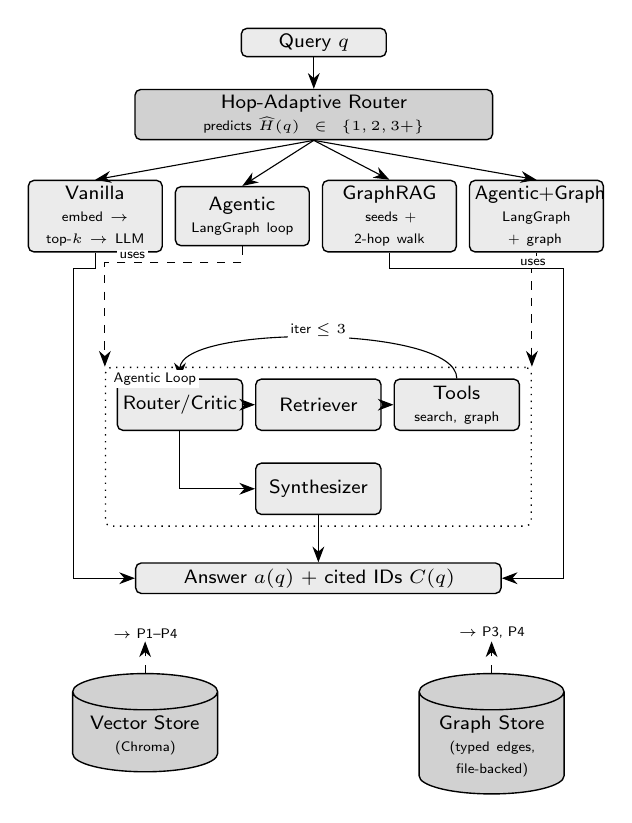
\begin{tikzpicture}[
  node distance=4mm,
  >={Stealth[length=2mm]},
  every node/.style={font=\sffamily\scriptsize}
]
\tikzset{
  box/.style    ={draw=black, line width=0.5pt, rounded corners=2pt,
                  align=center, inner sep=2pt},
  light/.style  ={box, fill=black!8},
  mid/.style    ={box, fill=black!18},
  pipe/.style   ={light, text width=1.55cm, minimum width=1.7cm,
                  minimum height=7.5mm},
  lp/.style     ={light, text width=1.45cm, minimum width=1.55cm,
                  minimum height=6.5mm},
  store/.style  ={cylinder, shape border rotate=90, aspect=0.25,
                  draw=black, line width=0.5pt, fill=black!18,
                  align=center, inner sep=2pt,
                  text width=1.7cm, minimum height=7mm},
  arr/.style    ={->, line width=0.4pt},
  darr/.style   ={arr, dashed},
  lab/.style    ={font=\sffamily\tiny, fill=white, inner sep=1pt},
  group/.style  ={draw=black, line width=0.5pt, rounded corners=2pt,
                  dotted, inner sep=4pt}
}

%% ----- Top: Query, Router -----
\node[light, text width=1.7cm] (q) at (0,0) {Query $q$};
\node[mid, below=4mm of q, text width=4.4cm] (router)
  {Hop-Adaptive Router\\{\tiny predicts $\widehat{H}(q) \in \{1, 2, 3{+}\}$}};
\draw[arr] (q) -- (router);

%% ----- Pipelines (centered at x=0) -----
\node[pipe, below=5mm of router, xshift=-2.775cm] (p1)
  {Vanilla\\{\tiny embed $\to$ top-$k$ $\to$ LLM}};
\node[pipe, right=1.5mm of p1] (p2)
  {Agentic\\{\tiny LangGraph loop}};
\node[pipe, right=1.5mm of p2] (p3)
  {GraphRAG\\{\tiny seeds + 2-hop walk}};
\node[pipe, right=1.5mm of p3] (p4)
  {Agentic+Graph\\{\tiny LangGraph + graph}};
\foreach \i in {1,2,3,4}
  \draw[arr] (router.south) -- (p\i.north);

%% ----- Agentic Loop subgraph (centered below pipelines) -----
\node[lp] (critic) at (-1.7,-4.6) {Router/Critic};
\node[lp, right=1.5mm of critic] (retr)  {Retriever};
\node[lp, right=1.5mm of retr]   (tools) {Tools\\{\tiny search, graph}};
\node[lp, below=4mm of retr]     (synth) {Synthesizer};

\draw[arr] (critic) -- (retr);
\draw[arr] (retr)   -- (tools);
\draw[arr] (tools.north) to[out=90,in=90,looseness=0.5]
  node[lab, midway, yshift=1mm] {iter $\le 3$} (critic.north);
\draw[arr] (critic.south) |- (synth.west);

\begin{scope}[on background layer]
  \node[group, fit=(critic)(retr)(tools)(synth)] (loop) {};
\end{scope}
\node[lab, anchor=north west]
  at ([xshift=2pt,yshift=-1pt]loop.north west) {Agentic Loop};

%% ----- P2, P4 -> Loop (dashed "uses"; right-angle elbows) -----
\draw[darr] (p2.south) -- ++(0,-2mm) -| (loop.north west)
  node[lab, pos=0.4, above] {uses};
\draw[darr] (p4.south) -- ++(0,-2mm) -| (loop.north east)
  node[lab, pos=0.4, above] {uses};

%% ----- Output -----
\node[light, below=6mm of synth, text width=4.5cm] (out)
  {Answer $a(q)$ + cited IDs $C(q)$};
\draw[arr] (synth.south) -- (out.north);

%% ----- P1, P3 -> Output (bypass loop on the sides) -----
\draw[arr] (p1.south) -- ++(0,-2mm) -|
  ([xshift=-4mm]loop.south west) |- (out.west);
\draw[arr] (p3.south) -- ++(0,-2mm) -|
  ([xshift=4mm]loop.south east)  |- (out.east);

%% ----- Data stores at the bottom; consolidated arrows -----
\node[store, below=10mm of out, xshift=-22mm] (s1)
  {Vector Store\\{\tiny (Chroma)}};
\node[store, below=10mm of out, xshift=22mm]  (s2)
  {Graph Store\\{\tiny (typed edges, file-backed)}};

\draw[darr] (s1.north) -- ++(0,4mm)
  node[lab, anchor=south] {$\to$ P1--P4};
\draw[darr] (s2.north) -- ++(0,4mm)
  node[lab, anchor=south] {$\to$ P3, P4};

\end{tikzpicture}

%%       so the figure renders inline when main.tex is compiled.
%%
%% Required preamble in the host document:
%%   \usepackage{tikz}
%%   \usetikzlibrary{positioning, arrows.meta, shapes.geometric,
%%                   fit, backgrounds, calc}

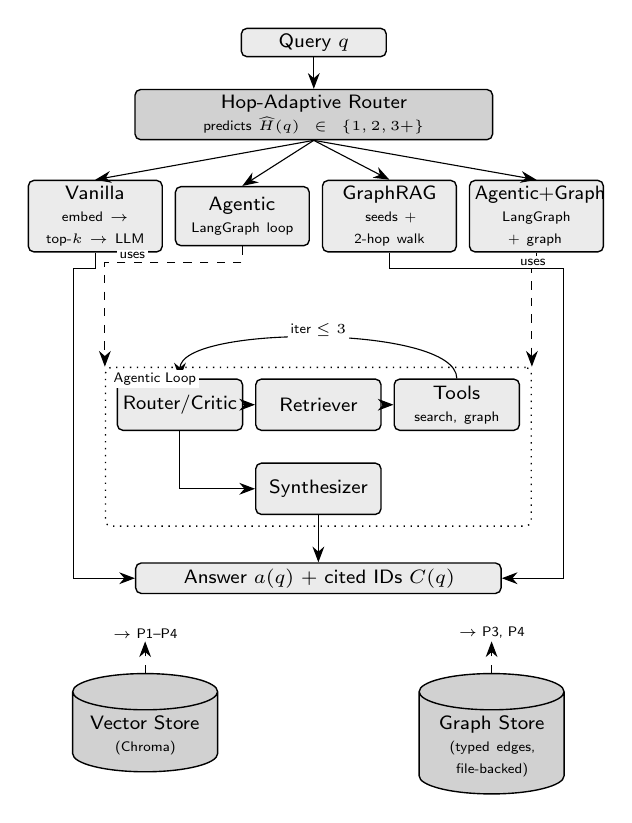
\begin{tikzpicture}[
  node distance=4mm,
  >={Stealth[length=2mm]},
  every node/.style={font=\sffamily\scriptsize}
]
\tikzset{
  box/.style    ={draw=black, line width=0.5pt, rounded corners=2pt,
                  align=center, inner sep=2pt},
  light/.style  ={box, fill=black!8},
  mid/.style    ={box, fill=black!18},
  pipe/.style   ={light, text width=1.55cm, minimum width=1.7cm,
                  minimum height=7.5mm},
  lp/.style     ={light, text width=1.45cm, minimum width=1.55cm,
                  minimum height=6.5mm},
  store/.style  ={cylinder, shape border rotate=90, aspect=0.25,
                  draw=black, line width=0.5pt, fill=black!18,
                  align=center, inner sep=2pt,
                  text width=1.7cm, minimum height=7mm},
  arr/.style    ={->, line width=0.4pt},
  darr/.style   ={arr, dashed},
  lab/.style    ={font=\sffamily\tiny, fill=white, inner sep=1pt},
  group/.style  ={draw=black, line width=0.5pt, rounded corners=2pt,
                  dotted, inner sep=4pt}
}

%% ----- Top: Query, Router -----
\node[light, text width=1.7cm] (q) at (0,0) {Query $q$};
\node[mid, below=4mm of q, text width=4.4cm] (router)
  {Hop-Adaptive Router\\{\tiny predicts $\widehat{H}(q) \in \{1, 2, 3{+}\}$}};
\draw[arr] (q) -- (router);

%% ----- Pipelines (centered at x=0) -----
\node[pipe, below=5mm of router, xshift=-2.775cm] (p1)
  {Vanilla\\{\tiny embed $\to$ top-$k$ $\to$ LLM}};
\node[pipe, right=1.5mm of p1] (p2)
  {Agentic\\{\tiny LangGraph loop}};
\node[pipe, right=1.5mm of p2] (p3)
  {GraphRAG\\{\tiny seeds + 2-hop walk}};
\node[pipe, right=1.5mm of p3] (p4)
  {Agentic+Graph\\{\tiny LangGraph + graph}};
\foreach \i in {1,2,3,4}
  \draw[arr] (router.south) -- (p\i.north);

%% ----- Agentic Loop subgraph (centered below pipelines) -----
\node[lp] (critic) at (-1.7,-4.6) {Router/Critic};
\node[lp, right=1.5mm of critic] (retr)  {Retriever};
\node[lp, right=1.5mm of retr]   (tools) {Tools\\{\tiny search, graph}};
\node[lp, below=4mm of retr]     (synth) {Synthesizer};

\draw[arr] (critic) -- (retr);
\draw[arr] (retr)   -- (tools);
\draw[arr] (tools.north) to[out=90,in=90,looseness=0.5]
  node[lab, midway, yshift=1mm] {iter $\le 3$} (critic.north);
\draw[arr] (critic.south) |- (synth.west);

\begin{scope}[on background layer]
  \node[group, fit=(critic)(retr)(tools)(synth)] (loop) {};
\end{scope}
\node[lab, anchor=north west]
  at ([xshift=2pt,yshift=-1pt]loop.north west) {Agentic Loop};

%% ----- P2, P4 -> Loop (dashed "uses"; right-angle elbows) -----
\draw[darr] (p2.south) -- ++(0,-2mm) -| (loop.north west)
  node[lab, pos=0.4, above] {uses};
\draw[darr] (p4.south) -- ++(0,-2mm) -| (loop.north east)
  node[lab, pos=0.4, above] {uses};

%% ----- Output -----
\node[light, below=6mm of synth, text width=4.5cm] (out)
  {Answer $a(q)$ + cited IDs $C(q)$};
\draw[arr] (synth.south) -- (out.north);

%% ----- P1, P3 -> Output (bypass loop on the sides) -----
\draw[arr] (p1.south) -- ++(0,-2mm) -|
  ([xshift=-4mm]loop.south west) |- (out.west);
\draw[arr] (p3.south) -- ++(0,-2mm) -|
  ([xshift=4mm]loop.south east)  |- (out.east);

%% ----- Data stores at the bottom; consolidated arrows -----
\node[store, below=10mm of out, xshift=-22mm] (s1)
  {Vector Store\\{\tiny (Chroma)}};
\node[store, below=10mm of out, xshift=22mm]  (s2)
  {Graph Store\\{\tiny (typed edges, file-backed)}};

\draw[darr] (s1.north) -- ++(0,4mm)
  node[lab, anchor=south] {$\to$ P1--P4};
\draw[darr] (s2.north) -- ++(0,4mm)
  node[lab, anchor=south] {$\to$ P3, P4};

\end{tikzpicture}
}%
  \caption{The five pipelines and their shared components. Vanilla and
    GraphRAG make a single synthesis call. Agentic and Agentic+Graph run
    a router, retriever, tool, and critic loop for at most three
    iterations before synthesis. The adaptive pipeline (rule-based V1 or
    learned V2) selects one of the four base pipelines per query.}
  \label{fig:architecture}
\end{figure}

\subsection{Pipelines}
\label{sec:pipelines}
All pipelines share the embedder, a ChromaDB vector store, a file-backed
typed-edge graph, the GPT-5.4 generator, and a grounded synthesis
prompt, so they differ only in how they retrieve
(Fig.~\ref{fig:architecture}).
\textbf{(i)~Vanilla} retrieves the top 10 chunks by dense similarity,
passes the top 5 to the synthesizer, and makes one synthesis call.
\textbf{(ii)~Agentic} is a LangGraph~\cite{langgraph_software} loop of
router, retriever, and critic with a single \texttt{search\_documents}
tool and at most three iterations.
\textbf{(iii)~GraphRAG} takes 8 vector seeds, walks up to two hops in
the typed graph (at most 30 nodes), and passes at most 15 chunks to one
synthesis call. It is a local-walk retriever in the GraphRAG family
rather than the community-summarisation system of Edge
et al.~\cite{graphrag2024}; we use ``GraphRAG'' as the family name.
\textbf{(iv)~Agentic+Graph} adds a typed \texttt{graph\_lookup} tool to
(ii). \textbf{(v)~Adaptive} chooses among (i) to (iv) for each query. We
evaluate a rule-based router (V1) and a learned router (V2), an
out-of-fold logistic regression over 11 text features and 3
principal components of the query embedding that sends each predicted
hop class to its empirically best pipeline.

\subsection{Experimental Factors}
\label{sec:axes}
\textbf{Embedder.} We use three models from three vendors at three
dimensionalities: e5-small (384 dimensions), OpenAI
text-embedding-3-small (1536), and BAAI bge-m3 (1024). The vector index is rebuilt per embedder; the graph is shared.
\textbf{Traversal.} Besides the bounded undirected walk (at most two
hops, at most 30 nodes), we run personalized PageRank from the same
vector seeds. It is unbounded in radius and ranks nodes by random-walk
mass, and all other settings are held fixed.
\textbf{Corpus.} The main corpus is a synthetic DO-178C-style
collection of 1{,}132 aerospace requirements in 30 modules (17 to 76
requirements per module; median length 59 tokens, 90th percentile 103).
GPT-5.4 generated it from a hand-authored module taxonomy, and we
release it with its link annotations. Retrieval traverses five
traceability edge types (\textit{derives\_from}, \textit{satisfies},
\textit{references}, \textit{verifies}, and \textit{refines}); we exclude
system-engineering edges such as allocation, which do not help
retrieval. Two Wikipedia corpora test transfer: 200 MuSiQue~\cite{musique2022}
questions (67, 67, and 66 of two, three, and four hops, mapped to our
three strata, with \textit{REFERENCES} edges between consecutive
supporting paragraphs) and 200 2WikiMultihopQA~\cite{twowiki2020}
questions, stratified by reasoning type: \textit{comparison} questions are one-hop,
\textit{compositional} and \textit{inference} questions are two-hop, and
\textit{bridge\_comparison} questions are three-or-more-hop.
\textbf{Judge.} Faithfulness is judged by GPT-5.4, GPT-4.1, and
Gemini 3.7-flash (Section~\ref{sec:experiments}).

\subsection{Queries and Gold Evidence}
\label{sec:queries}
We build the DO-178C queries from the graph rather than by free-form
prompting. We sample directed chains of one, two, and three to four
requirement links over the five edge types and prompt GPT-5.4 to phrase
one natural-language question that the chain answers. The nodes of the
chain form the gold evidence, so the gold set grows with the stratum
(on average 2.00, 3.00, and 4.68 IDs). This yields 296 queries (100,
99, and 97 per stratum), of which 85\% cross module boundaries; 497 of
the 655 chain edges are \textit{references} links. The gold sets are structural rather than human-annotated: a sampled
chain is a supporting path by construction, but we do not verify that
no other path answers the question. Citation recall is therefore exact
and precision conservative, equally for all pipelines.

\subsection{Metrics}
\label{sec:metrics}
We report citation precision, recall, and $F_1$ against the gold ID
sets, following ALCE~\cite{alce2023}. Cited IDs are parsed from the
answer text with a parser anchored to the corpus vocabulary, which
matches exact IDs and prefers the longest match. Hallucinated IDs that
reuse a real module prefix count against precision, and incidental
tokens such as SHA-256 or DO-254 are ignored. We report separately the context precision (the gold fraction of the
chunks handed to the synthesizer) and the retrieval recall, since
conflating context and citations changes which architecture appears to
win (Section~\ref{sec:c2}).

Each faithfulness judgment is a binary verdict, returned as strict JSON,
on whether the answer is supported by the retrieved context. For
agreement we report Cohen's $\kappa$, Gwet's
AC1~\cite{gwet2008,feinstein1990}, raw agreement, and an exact McNemar
test. For each faithfulness cell we report a Wilson 95\% confidence
interval and a Cochran--Armitage test for trend over hop depth. Three
same-judge controls (test--retest, embedder swap, and re-judging after
eleven weeks) use a paired subset of 300 tuples
(Section~\ref{sec:c4}).

\section{Experimental Setup}
\label{sec:experiments}

\noindent\textbf{Runs.} On DO-178C, we run 5 pipelines $\times$ 296 queries
$\times$ 3 seeds, giving 4{,}440 runs under each of two embedders
(e5-small, which we call \emph{v2}, and text-embedding-3-small,
\emph{v3}). We add 1{,}480 runs at one seed under bge-m3 (\emph{v4})
and a 296-run personalized PageRank arm under the v3 embedder. On
MuSiQue, we run vanilla, GraphRAG, and agentic+graph on 200 queries at
one seed (600 runs, v3 embedder), since RQ2 needs only these three, and
extend the GraphRAG arm to three seeds to match DO-178C's per-stratum
sample. On the same queries we add 400 runs for two mitigations and a
200-run GraphRAG control with distractor edges (Section~\ref{sec:c1}).
On 2WikiMultihopQA, we run vanilla and GraphRAG on 200 queries at three
seeds (1{,}200 runs, v3 embedder).

\noindent\textbf{Faithfulness judging.} On DO-178C, GPT-5.4 and GPT-4.1 judge
two disjoint stratified batches of 300 rows each (60 per pipeline;
seeds 42 and 43), the second eleven weeks after the first. Each batch is
fixed to the same 300 (query, pipeline, repeat) tuples across
embedders, so embedder differences are computed on identical items, and
batches judged on different dates are never pooled. In a later pass, GPT-4.1
and Gemini 3.7-flash judge every row of the DO-178C matrices and of the
Wikipedia corpora. Gemini judged four days after GPT-4.1 on DO-178C and
one day after it on the Wikipedia corpora, in both cases on the same
stored answer and context strings, so the pairing is exact at the row
level. Two same-input
controls re-judge 300 v2 tuples with GPT-5.4, once on the same day
(test--retest) and once eleven weeks later. A generator-swap control
re-synthesizes 332 v3 rows with GPT-4.1 on frozen retrievals and judges
them with both judges.

\noindent\textbf{Statistical protocol.} We compute 95\% BCa bootstrap
intervals~\cite{du2025bootstrap} with 1{,}000 resamples paired at the
query level, Wilcoxon signed-rank tests with Holm correction over the
30 contrasts of pipeline pair and stratum~\cite{bergkirkpatrick2012,koehn2004},
and Cliff's $\delta$, which we treat as negligible below 0.147. We call
two pipelines significantly different only when the BCa interval
excludes zero, the Holm-adjusted $p$ is below 0.05, and
$|\delta| \ge 0.147$. Tests pool the three seeds; we report the spread across seeds
separately (Section~\ref{sec:c1}).

\noindent\textbf{Reproducibility.} The original graph store was populated
before this study and contains edges beyond those annotated in the
released corpus. Loading the release with our ETL recovers 91.0\% of
the edges and 82.8\% of the chains behind our queries. Every gold set is
nevertheless exact, since the query manifest is released with its full
chains. The v2 and v3 graph arms walked the original store, while
the bge-m3 matrix and the PageRank arm walked a file-backed store built
from the released annotations, which is also what a reproduction uses.
To check that the change of graph does not drive our comparisons, we
rebuilt every v3 GraphRAG context on the file-backed store without
generation. The vector seeds are identical for 295 of the 296 queries,
the two contexts have a Jaccard overlap of 0.89, and context precision
(0.131 against 0.129) and retrieval recall (0.720 against 0.724) differ
by at most 0.01 in every stratum. We did not regenerate answers on the
new store, so the citation side of this check is untested.
We use the Azure snapshots \texttt{gpt-5.4-}\allowbreak\texttt{2026-03-05}
(generator and judge) and \texttt{gpt-4.1-2025-04-14} (judge) in
reasoning mode, with a completion cap of 8{,}192 tokens. The MuSiQue
subgraph (3{,}996 paragraph chunks and 399 \textit{REFERENCES} edges) is
built deterministically from the \texttt{dgslibisey} mirror (validation
split, seed 20260511), and the 2WikiMultihopQA subgraph (2{,}000 chunks
and 332 edges) from the \texttt{voidful} mirror (seed 20260816) by the
same procedure.

\section{Results}
\label{sec:results}

\begin{table*}[t]
  \centering
  \caption{Citation $F_1$ by hop stratum in four settings. v2 and v3: DO-178C with the e5-small and text-embedding-3-small embedders (4{,}440 runs each). MuSiQue: 200 queries with the v3 embedder (600 runs; vanilla, agentic+graph, and GraphRAG only). 2Wiki: 200 2WikiMultihopQA queries at three seeds (1{,}200 runs; vanilla and GraphRAG only). Bold marks the best pipeline per setting and stratum.}
  \label{tab:dominance}
  \footnotesize\setlength{\tabcolsep}{3pt}
  \resizebox{\textwidth}{!}{%
  \begin{tabular}{l ccc | ccc | ccc | ccc}
    \toprule
     & \multicolumn{3}{c|}{v2 main (local)} & \multicolumn{3}{c|}{v3 main (Azure)} & \multicolumn{3}{c|}{MuSiQue (Azure)} & \multicolumn{3}{c}{2Wiki (Azure)} \\
    System & 1h & 2h & 3+h & 1h & 2h & 3+h & 1h & 2h & 3+h & 1h & 2h & 3+h \\
    \midrule
    vanilla & \textbf{.757} & .712 & .089 & \textbf{.756} & .689 & .195 & .742 & .415 & .277 & \textbf{.990} & .778 & .678 \\
    agentic & .541 & .414 & .175 & .533 & .430 & .203 & --- & --- & --- & --- & --- & --- \\
    agentic-graph & .566 & .415 & \textbf{.219} & .547 & .421 & .251 & .457 & .296 & .249 & --- & --- & --- \\
    graphrag & .751 & \textbf{.720} & .172 & .745 & \textbf{.707} & .253 & \textbf{.841} & \textbf{.632} & \textbf{.463} & .969 & \textbf{.946} & \textbf{.938} \\
    adaptive & .630 & .499 & .181 & .651 & .492 & \textbf{.254} & --- & --- & --- & --- & --- & --- \\
    \bottomrule
  \end{tabular}}
\end{table*}


\begin{figure}[t!]
  \centering
  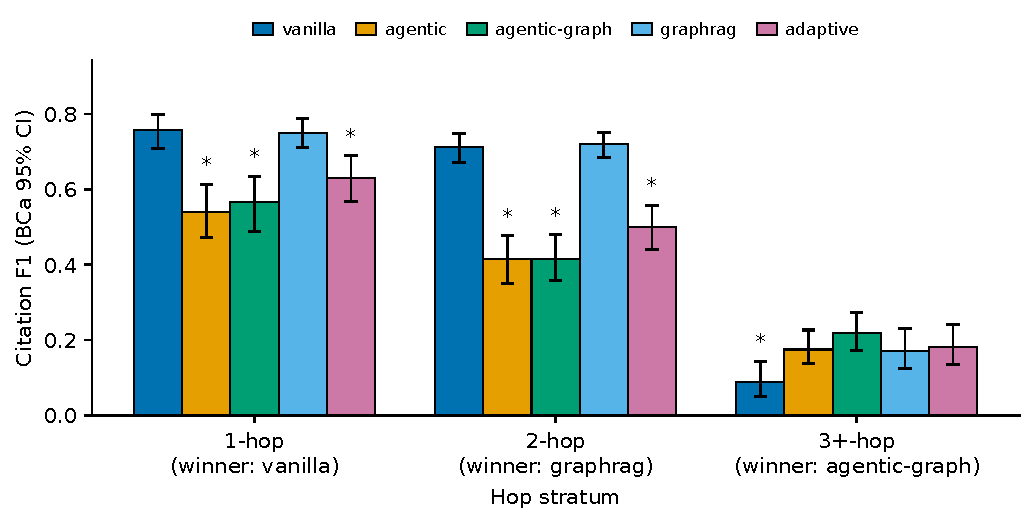
\includegraphics[width=0.55\textwidth]{figures/fig1_per_stratum_f1.pdf}
  \caption{Citation $F_1$ by hop stratum on the v2 matrix (DO-178C,
    e5-small), with 95\% BCa intervals. An asterisk marks a pipeline that
    differs significantly from the best pipeline in its stratum (Holm-adjusted
    Wilcoxon $p < 0.05$ and $|\delta| \ge 0.147$).}
  \label{fig:perstratum}
\end{figure}

\subsection{Citation Quality by Hop Depth (RQ1)}
\label{sec:c1}
Table~\ref{tab:dominance} reports citation $F_1$ by stratum in four
settings. On DO-178C, vanilla and GraphRAG are statistically tied on
one- and two-hop queries (Wilcoxon $p = 0.12$ and $0.65$ under the v2
embedder, with negligible $\delta$), and the agentic loop costs 0.19 to
0.30 $F_1$ on these strata. On queries of three or more hops the
ordering reverses. Vanilla falls to last place, and the pipelines that
use the graph lead; under the v2 embedder agentic+graph reaches 0.219
against 0.089 for vanilla (Holm $p < 10^{-6}$). Under the v3 embedder the ordering is the same, but no pair at this depth passes the joint criterion. Under bge-m3 the pattern recurs (Table~\ref{tab:embedders}):
vanilla is last at three or more
hops under all three embedders, and under bge-m3 both graph pipelines
outperform it by 0.100 and 0.091 (Holm $p = 2.1 \times 10^{-4}$ and
$1.4 \times 10^{-3}$), while the one- and two-hop contrasts remain
negligible.

On MuSiQue, GraphRAG is best in every stratum ($F_1$ of 0.841, 0.632,
and 0.463), with $p \le 5.1 \times 10^{-4}$ and $\delta$ between 0.27
and 0.43 against vanilla. Because the MuSiQue \textit{REFERENCES} edges
connect only gold paragraphs, we also ran GraphRAG on a graph with
additional edges between consecutive distractor paragraphs. GraphRAG
then loses 0.02, 0.05, and 0.09 $F_1$ per stratum and still outperforms
vanilla in every stratum ($p \le 0.014$), so its advantage on MuSiQue
does not depend on gold-only edges. On 2WikiMultihopQA, the two
pipelines are tied on one-hop queries ($p = 0.15$), and GraphRAG leads
on two-hop and deeper queries by 0.168 and 0.260 ($\delta = 0.48$ and
0.87). This is the DO-178C crossover again, on a graph we did not build.

Seed variation is small by comparison. The mean $F_1$ of each pipeline
changes by at most 0.031 between seeds,
every significant ordering holds in each seed separately, and the only
changes in rank occur between vanilla and GraphRAG on one- and two-hop
queries, which we already report as ties. Regarding RQ1, the best
pipeline depends on hop depth and on the corpus, but not on the embedder
or the seed.

\begin{table}[t]
  \centering
  \caption{Citation $F_1$ by hop stratum on DO-178C under three embedders from three vendors (e5-small, 384 dimensions; text-embedding-3-small, 1536; bge-m3, 1024). Bold marks the best pipeline per embedder and stratum.}
  \label{tab:embedders}
  \small
  \setlength{\tabcolsep}{4pt}
    \begin{tabular}{l rrr rrr rrr}
    \toprule
    & \multicolumn{3}{c}{e5-small (384d)} & \multicolumn{3}{c}{3-small (1536d)} & \multicolumn{3}{c}{bge-m3 (1024d)} \\
    \cmidrule(lr){2-4}\cmidrule(lr){5-7}\cmidrule(lr){8-10}
    System & 1h & 2h & 3+h & 1h & 2h & 3+h & 1h & 2h & 3+h \\
    \midrule
    vanilla       & \textbf{.757} & .712 & .089 & \textbf{.756} & .689 & .195 & \textbf{.769} & .691 & .114 \\
    agentic       & .541 & .414 & .175 & .533 & .430 & .203 & .548 & .404 & .156 \\
    agentic-graph & .566 & .415 & \textbf{.219} & .547 & .421 & .251 & .546 & .431 & .206 \\
    graphrag      & .751 & \textbf{.720} & .172 & .745 & \textbf{.707} & .253 & .742 & \textbf{.728} & \textbf{.214} \\
    adaptive      & .630 & .499 & .181 & .651 & .492 & \textbf{.254} & .672 & .478 & .202 \\
    \bottomrule
  \end{tabular}
\end{table}


\begin{table}[t]
  \centering
  \caption{Context and citation precision of GraphRAG in six settings. Slots: chunks passed to the synthesizer. IDs: IDs cited in the answer. Gain: citation precision divided by context precision.}
  \label{tab:pathology}
  \small
  \setlength{\tabcolsep}{4pt}
  \begin{tabular}{l rr rr r}
    \toprule
    & \multicolumn{2}{c}{\textit{retrieved context}} & \multicolumn{2}{c}{\textit{answer citations}} & \\
    \cmidrule(lr){2-3}\cmidrule(lr){4-5}
    Setting & slots & prec. & IDs & prec. & gain \\
    \midrule
    DO-178C, e5-small     & 14.9 & 0.120 & 4.9 & 0.480 & 4.0$\times$ \\
    DO-178C, 3-small      & 14.9 & 0.129 & 5.0 & 0.493 & 3.8$\times$ \\
    DO-178C, bge-m3       & 14.8 & 0.121 & 4.7 & 0.490 & 4.1$\times$ \\
    DO-178C, PPR walk     & 14.9 & 0.131 & 4.9 & 0.509 & 3.9$\times$ \\
    MuSiQue               & 11.2 & 0.227 & 3.4 & 0.654 & 2.9$\times$ \\
    2WikiMultihopQA       & 11.4 & 0.230 & 2.5 & 0.975 & 4.2$\times$ \\
    \bottomrule
  \end{tabular}
\end{table}


\begin{figure}[t!]
  \centering
  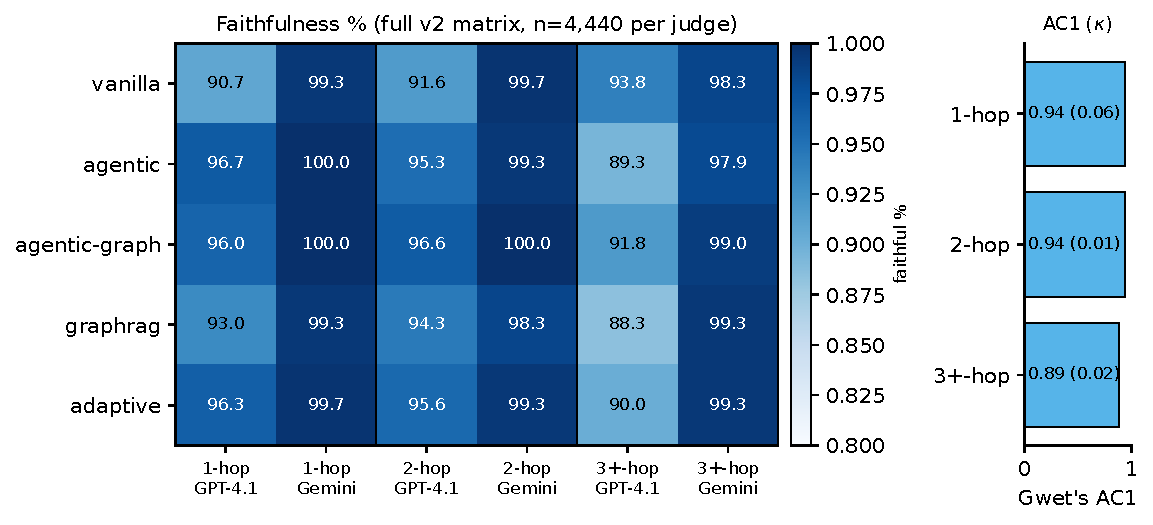
\includegraphics[width=0.8\textwidth]{figures/fig2_faithfulness_heatmap.pdf}
  \caption{Faithfulness on the full v2 matrix (DO-178C, e5-small; 4{,}440
    rows, about 300 per cell), judged by GPT-4.1 and Gemini 3.7-flash on
    the same rows. Left: percentage of answers judged faithful. Right:
    Gwet's AC1 between the two judges per stratum, with Cohen's $\kappa$
    in parentheses. The colour scale starts at 80\%.}
  \label{fig:faithheatmap}
\end{figure}

\subsection{Context Versus Answer Citations (RQ2)}
\label{sec:c2}
Table~\ref{tab:pathology} reports the same measurement in six settings,
covering three embedders, three corpora, and two traversals. GraphRAG's
walk fills 11 to 15 context slots at a context precision of 0.12 to
0.23, so four or five of every six chunks it retrieves are not gold. The
synthesizer then cites only 2.5 to 5.0 IDs per answer, at a citation
precision of 0.48 to 0.98. In every setting, the precision of the
citations is 2.9 to 4.2 times that of the context. The $F_1$ advantage
of GraphRAG is therefore a recall effect: the walk retrieves gold chunks
that dense retrieval misses, and the synthesizer does not cite most of
the irrelevant chunks that come with them.

An evaluation that scores the retrieved set as the attribution set, as
some GraphRAG comparisons do, sees only the first step and reaches the
opposite ranking. By context precision, GraphRAG
is below the vanilla baseline in every setting (0.12 to 0.23, against
0.27 to 0.37 for vanilla). By citation $F_1$, it is the best pipeline in
every setting, with scores of 0.551, 0.571, 0.565, 0.585, 0.646, and
0.951 in the row order of Table~\ref{tab:pathology}. 

Two controls test whether this depends on our design. The first
replaces the two-hop walk with personalized PageRank over the same
graph. Context
precision is 0.131 with PageRank and 0.129 with the original walk (0.131
for the walk rebuilt on the same file-backed graph;
Section~\ref{sec:experiments}). The precision gain from context to
citations is 3.9 and 3.8 times, and the difference in citation $F_1$ is
0.016 with $\delta = 0.036$, which our criterion treats as negligible.
The second control applies two mitigations on MuSiQue. Reranking the
walked neighbours by similarity to the query and keeping the top five
changes little (context precision from 0.227 to 0.232, citation $F_1$
$+0.010$, $p = 0.34$). Reducing the traversal budget from 30 to 10 nodes
and the context from 15 to 8 chunks lowers citation $F_1$ by 0.126
($p = 2.6 \times 10^{-11}$) and also lowers context precision, to 0.194.
Both outcomes fit a synthesizer that already filters: an upstream
filter adds little, and a smaller budget removes the recall the
advantage depends on. Regarding RQ2, the comparison
reverses with the measurement point in all six settings.

\subsection{Faithfulness and Hop Depth (RQ3)}
\label{sec:c3}
On 300-row judged subsets, faithfulness declines with hop depth on
DO-178C but not on the Wikipedia chains. This difference disappears at
adequate power. The MuSiQue arm had 67 rows per
stratum. Its drop from one-hop to three-or-more-hop queries (9.2
percentage points) was larger than the 4.7-point drop that is
significant on DO-178C, but detecting it with 80\% power requires about
210 rows per cell. With three seeds ($n = 600$), the decline is
significant under both judges, from 0.930 to 0.876 to 0.823 under GPT-4.1
($p = 1.1 \times 10^{-3}$) and from 0.955 to 0.945 to 0.869 under Gemini
($p = 1.2 \times 10^{-3}$). On 2WikiMultihopQA, judged in full
($n = 1{,}200$), faithfulness also declines ($p = 5.0 \times 10^{-2}$ and
$4.8 \times 10^{-6}$). The decline therefore replicates on all three
corpora under two vendors.

What distinguishes the pipelines is whether they expand the context.
Vanilla retrieves a fixed top five and adds nothing, and under GPT-4.1
it shows no significant drop from one-hop to three-or-more-hop queries.
Its change is $-1.5$ points on DO-178C ($n = 2{,}072$; $p = 0.16$, 0.99,
and 0.76 for the three embedders) and $+1.1$ points on 2WikiMultihopQA
($p = 0.66$). The four expanding pipelines drop by 6.3 and 6.7 points on
the same corpora (Fig.~\ref{fig:faithheatmap}). A logistic regression
of faithfulness on hop depth, an expansion indicator, and their
interaction turns this contrast into a single test. The interaction is
negative and significant on the pooled DO-178C matrix ($b = -0.599$,
$p = 1.0 \times 10^{-7}$, $n = 10{,}360$), and negative but not
significant on 2WikiMultihopQA ($b = -0.286$, $p = 0.27$), whose arm is
one twentieth the size.

Under Gemini the ordering is the same, but the test does not resolve.
Near the ceiling, vanilla itself shows a slope ($b = -0.729$,
$p = 0.012$), and the interaction cannot be separated from it
($p = 0.11$). The expanding pipelines still drop more than vanilla (2.8
against 1.5 points on DO-178C, 12.7 against 7.7 on 2WikiMultihopQA). A lenient judge preserves the ranking but not the power to test it
(Section~\ref{sec:c4}). Not every expanding pipeline declines in every cell: GraphRAG is
marginal under bge-m3 ($p = 0.065$), and the agentic pipelines decline
in four of six embedder and pipeline combinations. We have not re-run the GPT-5.4
judge at this sample size. Regarding RQ3, faithfulness declines with
hop depth on every corpus, and the decline is steeper for pipelines
that expand their context.

\begin{table}[t]
  \centering
  \caption{Judge agreement. Top: the same judge re-judging identical answer and context strings, so only the date differs. Middle: the same judge after an embedder swap changes the input. Bottom: GPT-4.1 against Gemini 3.7-flash on identical rows; the last column gives the fraction judged faithful by each.}
  \label{tab:judges}
  \small
  \setlength{\tabcolsep}{4pt}
    \begin{tabular}{l rrrr}
    \toprule
    \multicolumn{5}{l}{\textit{Same judge, frozen input (answer + context identical)}} \\
    \midrule
    GPT-5.4, re-judged same day & \multicolumn{4}{r}{$\kappa = 0.764$, raw agr.\ 0.88} \\
    GPT-5.4, re-judged 11 wk later & \multicolumn{4}{r}{$\kappa = 0.138$, raw agr.\ 0.56} \\
    GPT-4.1, re-judged 11 wk later & \multicolumn{4}{r}{$\kappa = -0.05\,/\,-0.00$ (v2/v3), raw agr.\ 0.48\,/\,0.51} \\
    GPT-4.1, full matrix vs.\ May & \multicolumn{4}{r}{$\kappa = -0.046$, raw agr.\ 0.48, $+43$\,pp} \\
    \midrule
    \multicolumn{5}{l}{\textit{Same judge, input changed by embedder swap}} \\
    \midrule
    GPT-5.4 (v2 vs v3) & \multicolumn{4}{r}{$\kappa = 0.137$, raw agr.\ 0.59} \\
    GPT-4.1 (v2 vs v3) & \multicolumn{4}{r}{$\kappa = 0.480$, raw agr.\ 0.74} \\
    \midrule
    \multicolumn{5}{l}{\textit{Cross-vendor, same rows (Gemini 3.7-flash vs.\ GPT-4.1)}} \\
    \midrule
    \textit{Setting} & raw & $\kappa$ & AC1 & faithful (G\,/\,4.1) \\
    \midrule
    DO-178C e5-small ($n{=}4{,}440$) & 0.929 & 0.029 & 0.923 & 0.993 / 0.933 \\
    DO-178C 3-small ($n{=}4{,}440$)  & 0.913 & 0.125 & 0.903 & 0.980 / 0.917 \\
    DO-178C bge-m3 ($n{=}1{,}480$)   & 0.939 & 0.047 & 0.935 & 0.991 / 0.945 \\
    DO-178C PPR walk ($n{=}296$)     & 0.926 & 0.058 & 0.919 & 0.983 / 0.936 \\
    MuSiQue, 3 seeds ($n{=}600$)     & 0.850 & 0.172 & 0.817 & 0.923 / 0.877 \\
    MuSiQue rerank ($n{=}200$)       & 0.820 & 0.171 & 0.772 & 0.935 / 0.825 \\
    MuSiQue budget cap ($n{=}200$)   & 0.875 & 0.419 & 0.841 & 0.875 / 0.880 \\
    2WikiMultihopQA ($n{=}1{,}200$)  & 0.899 & 0.435 & 0.877 & 0.888 / 0.914 \\
    \bottomrule
  \end{tabular}
\end{table}


\subsection{Judge Stability (RQ4)}
\label{sec:c4}
Table~\ref{tab:judges} separates instability on fixed inputs from
instability after the retrieval state changes.
\textit{Fixed inputs.} Re-judging the same 300 stored answer and
context pairs gives GPT-5.4 a self-agreement of $\kappa = 0.76$ (raw
agreement 0.88) on the same day, but only $\kappa = 0.14$ (raw agreement
0.56) eleven weeks later, with 15 points more answers judged faithful.
This rejects a stationary judge (binomial $p < 10^{-44}$). GPT-4.1 on the same tuples agrees with its own earlier
verdicts only at chance level ($\kappa = -0.05$ and $-0.00$ for v2 and
v3) and judges 41 points more answers faithful. With fixed inputs, this is drift of the judge alone.
\textit{Changed retrieval state.} After an embedder swap, which
changes the context and the answer for 94\% of the tuples, GPT-5.4
changes 41\% of its verdicts ($\kappa = 0.137$) and GPT-4.1 changes 26\%
($\kappa = 0.48$). The judge that is more stable under the embedder
swap is thus the less stable over time.
\textit{Across vendors.} On the same rows, Gemini 3.7-flash is much
more lenient than GPT-4.1 on all four DO-178C settings (0.98 to 0.99
against 0.92 to 0.95 faithful; McNemar $p < 10^{-9}$). They are indistinguishable on the budget-capped MuSiQue arm (0.875 against 0.880,
$p = 1.00$), and Gemini is stricter on 2WikiMultihopQA (0.888 against
0.914, $p = 6.2 \times 10^{-3}$). Strictness is therefore a property of
the judge and corpus together, and a calibration offset measured on one
corpus cannot be reused on another. The same eight
settings show the prevalence paradox~\cite{feinstein1990} within one
pair of judges. Raw agreement ranges only from 0.82 to 0.94, and Gwet's
AC1 follows it (0.77 to 0.94), whereas $\kappa$ ranges from 0.03 to
0.44, ordered almost exactly by the distance of faithfulness from the
ceiling. On 2WikiMultihopQA the two judges agree less often than on
DO-178C (0.899 against 0.93), yet their $\kappa$ is fifteen times
higher (0.435 against 0.029). Leniency and trend are nevertheless
separate properties. Although Gemini is near the ceiling on DO-178C, it
reproduces the decline with hop depth on both DO-178C matrices
($p = 4.3 \times 10^{-3}$ and $p < 10^{-16}$) and on both Wikipedia
corpora. The ordering a judge induces replicates across vendors, while
its strictness does not.
\textit{Between judges.} Inter-judge agreement halves under the embedder swap ($\kappa$ from
0.30 to 0.17; McNemar $p < 0.001$), and on the 300-row MuSiQue batch
GPT-5.4 and GPT-4.1 agreed only at chance (raw agreement 0.48, AC1
0.08), a real disagreement rather than a prevalence effect. We therefore
re-judged the full matrix within one judging period
(Section~\ref{sec:c3}), and no comparison we report spans judging
dates. Regarding RQ4, judges are not stable over
time, across retrieval states, or across vendors, although the hop-wise
ordering they induce is.

\section{Discussion}
\label{sec:discussion}

\paragraph{Why expansion lowers faithfulness.}
The synthesizer leaves most irrelevant chunks out of its citations
(Section~\ref{sec:c2}), but they can still influence the answer. Because faithfulness is judged
against the full retrieved context, every chunk the walk adds is one
more chunk the answer can be judged unfaithful to. This mechanism does not depend on what the edges connect, consistent
with the decline on both typed DO-178C links and Wikipedia paragraph
links. The cost appears to scale with the number of added chunks
rather than with their relevance, since reranking them by relevance
changes nothing (Section~\ref{sec:c2}).

\paragraph{Implications for LLM judges.}
Since judges change with the retrieval state and the date
(Section~\ref{sec:c4}), single-judge comparisons of retrieval modules
are conditional on both, and ensembles help only partially. At a
minimum, faithfulness should be compared on paired tuples under a fixed
embedder and judged within one period.

\paragraph{Threats to validity.}
\emph{Construct validity.} Citation $F_1$ does not measure the quality
of the reasoning, so we pair it with faithfulness judgments, which are
themselves subject to bias~\cite{selfpref_bias2024,wallat2024}. We
quantify this bias directly (Section~\ref{sec:c4}) and use a third
judge from a different vendor on every matrix.
\emph{External validity.} The DO-178C corpus is a single synthetic
dataset, generated by the same model family that answers and judges,
and its absolute $F_1$ levels may not transfer to other regulated
domains. When GPT-4.1 re-synthesizes 332 answers on frozen retrievals, the
pipeline ordering and the faithfulness decline both hold, so neither
result is specific to GPT-5.4. The corpus, however, is still written by that family. The two Wikipedia
corpora, judged in full by two vendors, are our main check of external
validity; both reproduce the RQ1 crossover, although only DO-178C
includes all five pipelines. Our GraphRAG pipeline is one
local-walk implementation. Replacing the walk with personalized
PageRank leaves the RQ2 result unchanged, but a full third-party
GraphRAG system may flood or filter its context differently. The two
unsupervised mitigations we tried did not help, and a learned evidence
selector conditioned on the question remains to be tested.
\emph{Statistical conclusion validity.} Per-stratum samples for the citation metrics (97 to 100 queries on
DO-178C, 66 to 67 on Wikipedia) are at the lower end of BCa stability
under strong skew, but percentile intervals give the same conclusions. Faithfulness cells hold about 300 rows after full-matrix judging. The
hop-by-expansion interaction is significant on DO-178C, but on the much
smaller 2WikiMultihopQA arm we can report only its direction.

\paragraph{Artifact availability.}
The corpus with its link annotations, the query manifest with full
chains, the code, and every scored and judged CSV file are released
under CC-BY-4.0 \ifanonymous (links withheld for review)\else at
\url{https://huggingface.co/datasets/meftun/aerosys-requirements} and
\url{https://github.com/mftnakrsu/rag-vs-agentic}\fi. The Wikipedia
subsets are rebuilt by seeded scripts.

\section{Conclusion}
\label{sec:conclusion}
In this paper, we compared five RAG pipelines for multi-hop
requirements traceability while varying the embedder, corpus, graph
traversal, and judge. The citation measurement point reverses the
GraphRAG comparison in all six settings, the best pipeline per hop
depth is stable across embedders and seeds, and the faithfulness
decline follows context expansion on all three corpora. LLM judges
drift on identical inputs but agree on the hop-wise ordering. RAG
comparisons should therefore state their measurement point and report
results across these factors; testing a learned evidence selector and a
third-party GraphRAG system are natural next steps.


\bibliographystyle{splncs04}
\bibliography{refs}

\end{document}
